\section{Story Patterns (Christian und Marie)} \label{sec:StoryPatterns}

In this section, we introduce story patterns in more detail.
We start by giving the general idea of story patterns in Section \ref{sec:StoryPatterns:storyPattern}.
Thereafter, we describe the basic concepts of story patterns, namely object variables, link variables,
and their respective binding semantics in Sections \ref{sec:StoryPatterns:objects} to \ref{sec:StoryPatterns:binding}.
Finally, we show the use of object attributes in a story pattern in Section \ref{sec:StoryPatterns:attributes}.


\subsection{General Idea [CH]}
\label{sec:StoryPatterns:storyPattern}

Story patterns are typed attributed graph transformation rules with inheritance on object types (cf. Section \ref{sec:foundations:typedAttrGTS}) that may be embedded into an activity node of a story diagram (cf. Section \ref{sec:StoryDiagrams}).
 By using a type model as introduced in Section \ref{sec:typeGraph}, story patterns enable inheritance and polymorphism for matching object and link variables.
This allows for specifying graph replacement rules for object-oriented models.

As for normal graph transformations, object and link variables are matched to the objects and links of the instance model. 
In contrast to typed attributed graph transformation, story patterns explicitly require to use isomorphic matchings, i.e., two object variables of a story pattern may not be matched to the same object of the instance model.

For enabling a concise notation of the graph transformation, story patterns apply a short-hand notation depicting the left-hand side (LHS) and the right-hand side (RHS) in a single, annotated graph. 
Objects and links being created (or deleted) are annotated with \create (or  \destroy, respectively). 
Objects which are preserved by the graph transformation carry no annotation.
Then, the LHS consists of all objects that are preserved and deleted, while the RHS consists of all objects that are preserved and created. 
The deletion of objects follows the single pushout approach (cf.\ Section~\ref{sec:foundations:simpleGTS}).

Figure \ref{fig:simpleStoryPattern} shows an example of a single story pattern that redirects a method call from an old method to a new method.

\begin{figure}[htbp]
  \centering
  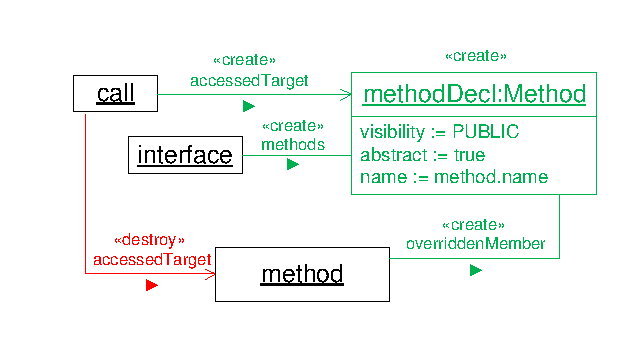
\includegraphics[scale=1.0]{figures/SimpleStoryPattern}
  \caption{Example of a Story Pattern}
  \label{fig:simpleStoryPattern}
\end{figure}

In the example, the object variables \fe{parentClass}, \fe{oldMethod}, and \fe{newMethod} are bound variables, i.e., they already refer to objects of the instance model (cf. Section \ref{sec:StoryPatterns:binding:states}).
The object variables \fe{anyMethod} and \fe{call} are unbound. 
When applying the story pattern, first a match for \fe{anyMethod} and \fe{call} is searched in the instance graph. 
A possible match will be any method in \fe{parentClass} which contains a call to \fe{oldMethod}. 
If the matching is successful, the link from \fe{c} to \fe{oldMethod} will be deleted and the link from \fe{c} to \fe{newMethod} will be created.

In our concrete syntax, the object and link variables which are not changed by the story pattern are visualized in black. 
Object and link variables to be destroyed are annotated with \destroy and visualized in red. 
Object and link variables to be created are annotated with \create and visualized in green. 
An unbound object variable is labeled with its name and the name of the corresponding type. 
For bound object variables, we omit the name of the type (e.g.\ \fe{parentClass} in Figure~\ref{fig:simpleStoryPattern}).

In general, the matching process is executed as a three step process:
first, a matching is searched which uses a bound variable of the story pattern as a starting point. 
The matching includes all objects and links not to be changed as well as all objects and links annotated with \destroy. 
If such a matching can be obtained, the story pattern is applicable and the execution proceeds. 
Otherwise the execution of the story pattern is aborted.
In the second step, all objects and links annotated with \destroy are deleted. 
Finally, in Step 3 all objects and links annotated with \create are created and added to the instance graph.

\subsection{Objects and Object Variables [MCP]}
\label{sec:StoryPatterns:objects}

Object variables represent the objects to be matched in a story pattern.
The variables are identified by their name.
The objects are instances of classes of the underlying type graph (cf.
Section \ref{sec:foundations:typedAttrGTS}). Thus, the object variables are typed by classes from this model, i.e.
EClass.

The story pattern in Figure \ref{fig:simpleStoryPattern} contains five
object variables with the names \fe{parentClass}, \fe{oldMethod}, \fe{anyMethod}, \fe{c} and
\fe{newMethod}. 
The type of an object variable is only visualized if the
variable is unbound or maybe bound (cf.\ Section
\ref{sec:StoryPatterns:binding:states}). For example, the object variable \fe{anyMethod} has the type \fe{Method}.

Object variables have binding states, binding operators and binding semantics.
They are described in Section  \ref{sec:StoryPatterns:binding}.


\ext %--- Comment this line to include primitive variables into the document
{
\todomcp{Primitive Variables: concrete syntax like
object variables; binding expressions for initialization, see figure
\ref{fig:primitiveVariable}; primitive variables are typed over EDataType; they
exist to the end of the Activity}

\begin{figure}[htbp]
  \centering
  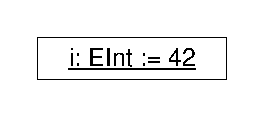
\includegraphics[scale=0.6]{figures/PrimitiveVariable}
  \caption{Primitive variable with value assignment}
  \label{fig:primitiveVariable}
\end{figure}

\todomcp{Links to primitive variables: special LinkVariable, typed over
EStructuralFeature}
}%------ End of primitive variables section



\subsection{Links and Link Variables [MCP]}
\label{sec:StoryPatterns:links}

Link variables represent connections between objects and are used to connect
different object variables. A link variable is typed over an EReference object of the underlying
type graph.

Like object variables, link variables also have binding
operators and binding semantics (cf. Section \ref{sec:StoryPatterns:binding}).




\subsection{Binding of Variables [MCP]}
\label{sec:StoryPatterns:binding}

Object variables and link variables have binding states (unbound, bound, maybe
bound), binding semantics (mandatory, negative, optional), and binding operators
(check only, create, destroy).


\subsubsection{Binding States}
\label{sec:StoryPatterns:binding:states}
An object variable or a link variable can be declared as bound, unbound, or
maybe bound (i.e. it is unknown if the variable is bound or not). This is
defined by its binding state. An unbound variable is matched during the
execution of the containing story pattern. 
Even if a variable of the same name was already matched earlier in the story diagram, the
pattern matching algorithm is forced to find a new object for this variable.
A bound variable must have been matched previously. 
For a variable that is specified as maybe bound, a new match will only be
determined if it has not been bound before. 
Otherwise it will be treated as a bound variable.
This is useful, if the same pattern should be used in different contexts, i.e., the bound variable of the pattern differs depending on the context but otherwise the patterns are identical.
Without maybe bound variables, different patterns would have to be modeled that only differ in which variable is the bound variable of the pattern.
With maybe bound variables, all variables can be set to maybe bound and the caller specifies a binding for one of them depending on the context.
%\todomcp{explain why maybe bound is necessary}
The variable scope is limited by the surrounding activity. 
That means, a bound variable keeps its binding until the activity ends, unless
it is matched again in the meantime.
An exception is the variable scope inside an each activity node (cf.\ Section
\ref{sec:storydiagrams:activitynodes}).

Unbound object variables are visualized with an underlined label of the form
``name: type'' while the type is hidden for bound object variables as depicted
in Figure \ref{fig:bindingStatesOverview} a) and b).
Maybe bound object variables are represented like unbound object variables but
are marked by a question mark after the name (cf.\ Figure
\ref{fig:bindingStatesOverview} c)).

In a valid, executable story pattern, each connected component\footnote{With
``connected component'' we mean a subgraph in which each object variable is
reachable from all other object variables via link variables.}
must contain at least one bound object variable or only created variables. This
is necessary to avoid a search over the whole underlying instance model which requires a long runtime in most cases.


\begin{figure}[htbp]
  \centering
  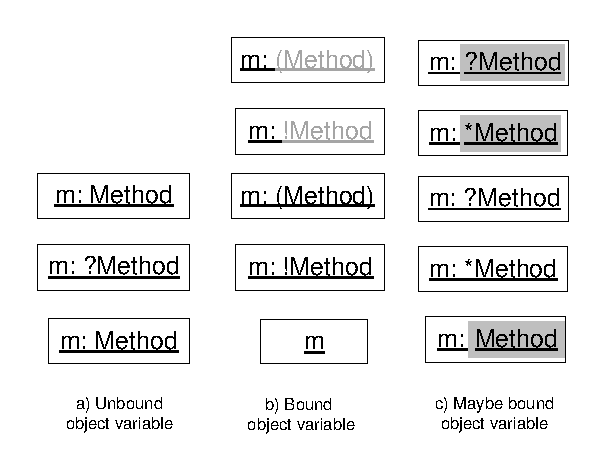
\includegraphics[scale=1.2]{figures/BindingStatesOverview}
  \caption{Binding States for object variables}
  \label{fig:bindingStatesOverview}
\end{figure}

\subsubsection{Binding Semantics}
\label{sec:StoryPatterns:binding:semantics}
Object variables and link variables have binding semantics that
determine if a variable is mandatory, negative or optional.
A match for mandatory variables must exist in the given instance model, otherwise
the pattern matching fails. 
In contrast, negative variables constitute so-called negative application
conditions and must not exist in the instance model. If a variable defined as
negative can be matched during the execution of the story pattern, the pattern
fails, too. Optional variables may exist. If an optional variable exists, it will be
bound, but if it does not exist, the story pattern may also be matched
successfully and execution proceeds.

Negative object variables are visualized crossed-out (cf. Figure
\ref{fig:bindingSemanticsOverview} b)) and optional object variables are
visualized with a dashed border (cf.\ Figure \ref{fig:bindingSemanticsOverview} c)).
The same holds for negative and optional link variables (cf. Figure
\ref{fig:bindingSemanticsOverview} e) and f)).

Negative and optional object variables and link variables are not part of a
connected component.
Optional and negative link variables do not represent
valid connections while optional and negative
object variables do not represent valid connection points. 
This means, the graph has to be still connected when ignoring optional and negative
parts. Consequently, regarding the rule that each connected component must
contain at least one bound object variable (cf.\ Section
\ref{sec:StoryPatterns:binding:states}), there are situations in which the
use of negative or optional object variables is not allowed. 
Figure \ref{fig:negativeObjects} shows example situations of this. 
For example, case a) is allowed but case b) is not because in the latter case
the graph without the negative and optional elements is not a connected component anymore.
Case c) is allowed because the object
variables \fe{a} and \fe{c} are bound which means that each connected component has at least one bound object variable.
Accordingly, case d) is allowed, too, because \fe{a} and \fe{b} are both
bound. Case e) is not allowed while Case f) is.
Case g) is not allowed since the semantics is the same as in case a) due to the single pushout approach of story patterns.

Similar to the application of negative object
variables, Figure \ref{fig:optionalObjects} shows some examples for the application of optional object variables. 
While case a) is allowed, case b) is not allowed because in this case the
shown graph is not connected any more. However, case c) and d) are allowed
because each connected component contains at least one bound object variable.
Case e) and f) are also allowed.

\begin{figure}[htbp]
  \centering
  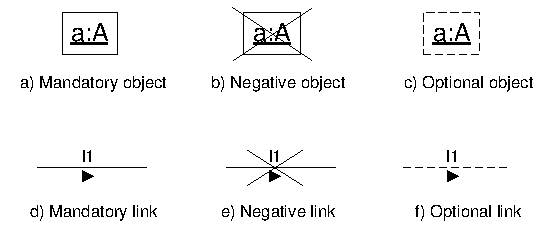
\includegraphics[scale=1.2]{figures/BindingSemanticsOverview}
  \caption{Binding Semantics for object and link variables}
  \label{fig:bindingSemanticsOverview}
\end{figure}

\begin{figure}[htbp]
  \centering
  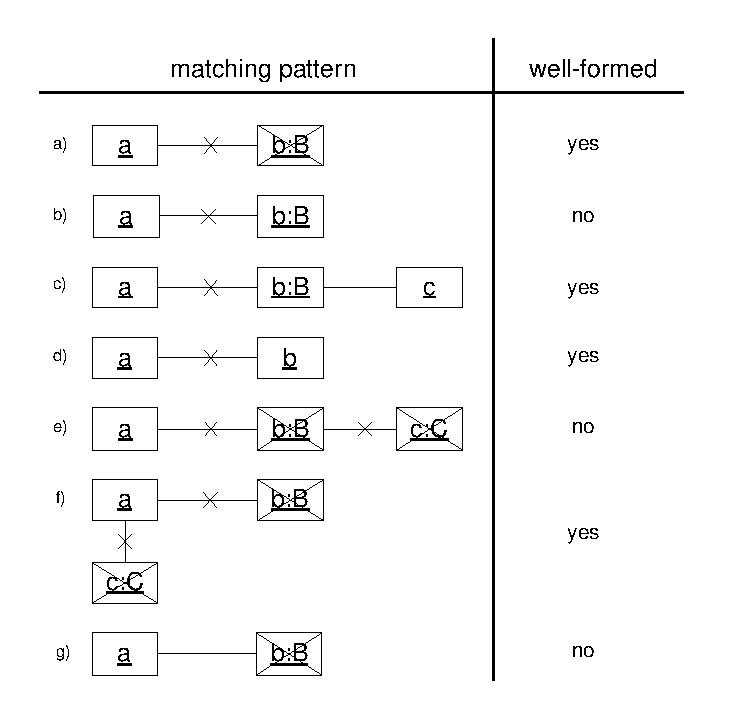
\includegraphics[scale=1]{figures/negativeObjects}
  \caption{Negative Application Conditions}
  \label{fig:negativeObjects}
\end{figure}

\begin{figure}[htbp]
  \centering
  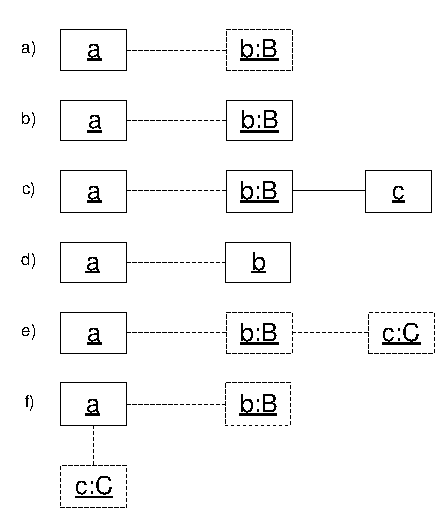
\includegraphics[scale=1]{figures/optionalObjects}
  \caption{Optional Object Variables}
  \label{fig:optionalObjects}
\end{figure}

\subsubsection{Binding Operators}
\label{sec:StoryPatterns:binding:operators}
Binding operators define whether an element or link is to be created, deleted,
or just matched (found).
After all elements that are defined to be deleted or just matched have been
matched, the model is modified by deleting and creating the elements as
defined (see Section~\ref{sec:StoryPatterns:storyPattern}).

Elements to be created are marked with the
label \create (cf.\ Figure \ref{fig:bindingOperatorsOverview} b) and e)) and elements
to be deleted are marked with the label \destroy (cf.\ Figure
\ref{fig:bindingOperatorsOverview} c) and f)).

\begin{figure}[htbp]
  \centering
  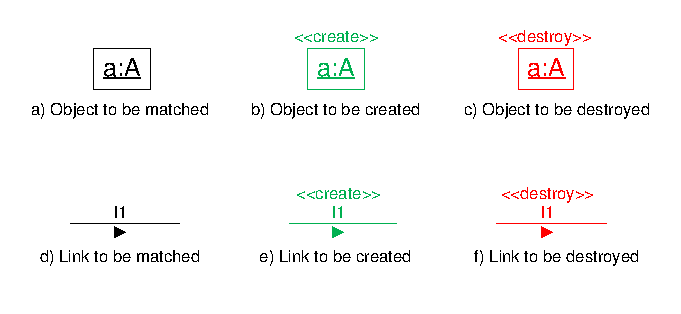
\includegraphics[scale=1.2]{figures/BindingOperatorsOverview}
  \caption{Binding Operators for object and link variables}
  \label{fig:bindingOperatorsOverview}
\end{figure}

Since elements marked with \create do not exist in the object graph during the
matching process yet, they also do not belong to a connected component (like
negative or optional variables).


\subsubsection{Feasible Binding Combinations}

Binding states, binding semantics and binding operators can be
arbitrarily combined, but only certain combinations are feasible. 
Table \ref{tab:bindingCombinations} lists all feasibly binding combinations for
object variables. As shown there, bound and maybe bound object variables must not have negative
or optional binding semantics. As well, the combination of the binding states
bound or maybe bound and the binding operator create is not allowed.

% Table generated by Excel2LaTeX from sheet 'Tabelle1'
\begin{table}[htbp]
  \centering
  \caption{Feasible combinations of binding states, binding semantics, and
  binding operators for object variables}
    \begin{tabular}{|r|r|r|r|}
    \hline
    \textbf{Binding State} & \textbf{Binding Semantics} & \textbf{Binding
    Operator} & \textbf{Feasible} \\
    \hline
    UNBOUND & MANDATORY & CHECK\_ONLY & yes \\
    UNBOUND & MANDATORY & CREATE & yes \\
    UNBOUND & MANDATORY & DESTROY & yes \\
    UNBOUND & NEGATIVE & CHECK\_ONLY & yes \\
    UNBOUND & NEGATIVE & CREATE & no \\
    UNBOUND & NEGATIVE & DESTROY & no \\
    UNBOUND & OPTIONAL & CHECK\_ONLY & yes \\
    UNBOUND & OPTIONAL & CREATE & yes \\
    UNBOUND & OPTIONAL & DESTROY & yes \\
    \hline
    BOUND & MANDATORY & CHECK\_ONLY & yes \\
    BOUND & MANDATORY & CREATE & no \\
    BOUND & MANDATORY & DESTROY & yes \\
    BOUND & NEGATIVE & CHECK\_ONLY & no \\
    BOUND & NEGATIVE & CREATE & no \\
    BOUND & NEGATIVE & DESTROY & no \\
    BOUND & OPTIONAL & CHECK\_ONLY & no \\
    BOUND & OPTIONAL & CREATE & no \\
    BOUND & OPTIONAL & DESTROY & no \\
    \hline
    MAYBE\_BOUND & MANDATORY & CHECK\_ONLY & yes \\
    MAYBE\_BOUND & MANDATORY & CREATE & no \\
    MAYBE\_BOUND & MANDATORY & DESTROY & yes \\
    MAYBE\_BOUND & NEGATIVE & CHECK\_ONLY & no \\
    MAYBE\_BOUND & NEGATIVE & CREATE & no \\
    MAYBE\_BOUND & NEGATIVE & DESTROY & no \\
    MAYBE\_BOUND & OPTIONAL & CHECK\_ONLY & no \\
    MAYBE\_BOUND & OPTIONAL & CREATE & no \\
    MAYBE\_BOUND & OPTIONAL & DESTROY & no \\
    \hline
    \end{tabular}%
  \label{tab:bindingCombinations}%
\end{table}%

%\todomcp{see albert's habil for example for optional-create}

%\todomcp{table for object set variables?}

\begin{table}[htbp]
  \centering
  \caption{Feasible combinations of binding semantics and
  binding operators for link variables}
    \begin{tabular}{|r|r|r|}
    \hline
    \textbf{Binding Semantics} & \textbf{Binding
    Operator} & \textbf{Feasible} \\
    \hline
    MANDATORY & CHECK\_ONLY & yes \\
    MANDATORY & CREATE & yes \\
    MANDATORY & DESTROY & yes \\
    NEGATIVE & CHECK\_ONLY & yes \\
    NEGATIVE & CREATE & no \\
    NEGATIVE & DESTROY & no \\
    OPTIONAL & CHECK\_ONLY & yes \\
    OPTIONAL & CREATE & yes \\
    OPTIONAL & DESTROY & yes \\
    \hline
    \end{tabular}%
  \label{tab:bindingCombinations_links}%
\end{table}%

The feasible combinations of binding semantics and binding operators for link
variables are given in Table \ref{tab:bindingCombinations_links}. Link variables
have no binding state.


\subsection{Using Object Attributes [CH]}
\label{sec:StoryPatterns:attributes}

The objects of our instance model carry attributes. 
During the application of a story pattern, these attributes can be used twofold. 
First, attribute constraints can be specified to restrict the attribute values to a certain range thereby restricting the possible matches of a story pattern. 
Second, attribute values can be changed during the graph rewriting step after a successful matching.

We use \emph{attribute constraints} to restrict the matching of object variables to objects of the instance model that have specific attribute values. 
Thus, attribute constraints are considered to be part of the LHS and do not change the instance model. 
Figure \ref{fig:objectConstraint} shows an example.

\begin{figure}[htbp]
  \centering
  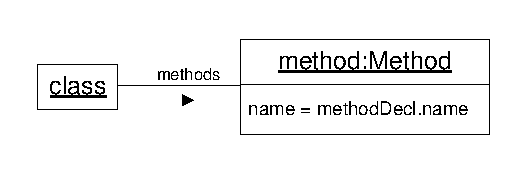
\includegraphics[scale=1]{figures/ObjectConstraint}
  \caption{Matching Pattern with an Attribute Constraint}
  \label{fig:objectConstraint}
\end{figure}

In the example, we match a method being contained in the class represented by the object variable \fe{theClass}. 
The match is restricted to a method which has the name "getName".

The values of attributes that are not restricted by an attribute constraint are not considered during the matching. 
Thus, they may have an arbitrary value. 
In the current version of story patterns, attribute constraints need to be specified using OCL~\cite{OCL}. 
Besides equality checks, all comparative operations on the attributes of the object supported by OCL can be used as object constraints. 

Beside attribute constraints, \emph{attribute assignments} may be used to change the value of an attribute during the application of a story pattern. 
Thus, attribute assignments are considered to be part of the RHS. 
When using attribute assignments, the value of the attribute is not considered while matching the LHS to the instance model. 
Figure \ref{fig:attributeAssignment} shows an example.

\begin{figure}[htbp]
  \centering
  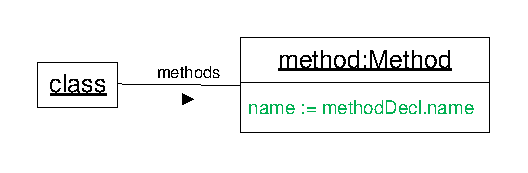
\includegraphics[scale=1]{figures/AttributeAssignment}
  \caption{Using an Attribute Assignment}
  \label{fig:attributeAssignment}
\end{figure}

In the example, the story pattern matches a method in class \fe{theClass} with an arbitrary name. 
Then, the name of the method is changed to \emph{"getMethodName"}. 

The concrete syntax of an attribute assignment is
\begin{lstlisting}
 <attributeAssignment> ::= #Attribute.name ':=' OCLExpression
\end{lstlisting}
The expression is to be specified using OCL. 
The type of the return value of the OCL expression must be the same as the type of the attribute. 
Since the attribute assignment is considered to be part of the RHS, it is visualized in green color.

The OCL statements we allow for attribute constraints and attribute assignments must not traverse the references of the object variables.
Both may only use the attributes of object variables in the story pattern and arbitrary arithmetic operations on them. 


\ext  %--- Comment this line to include object sets into the document
{
\subsection{Object Sets [MCP]}
\label{sec:StoryPatterns:objectsets}

explain objectSetVariables, set size expressions

\todomcp{object sets and binding operators/states/semantics}

\todomcp{If we bind an object set, can we use the bound object in other story pattern? E.g. to insert all elements bound by the object set into a container via a containment link? (See Figure \ref{fig:reuseObjSet}).}
\tododt{Yes, but I would use another concrete syntax (see Figures~\ref{fig:reuseObjSet1}, \ref{fig:reuseObjSet2}, and \ref{fig:reuseObjSet1}).}

\begin{figure}[p]
	\begin{minipage}{.45\textwidth}
		\centering
		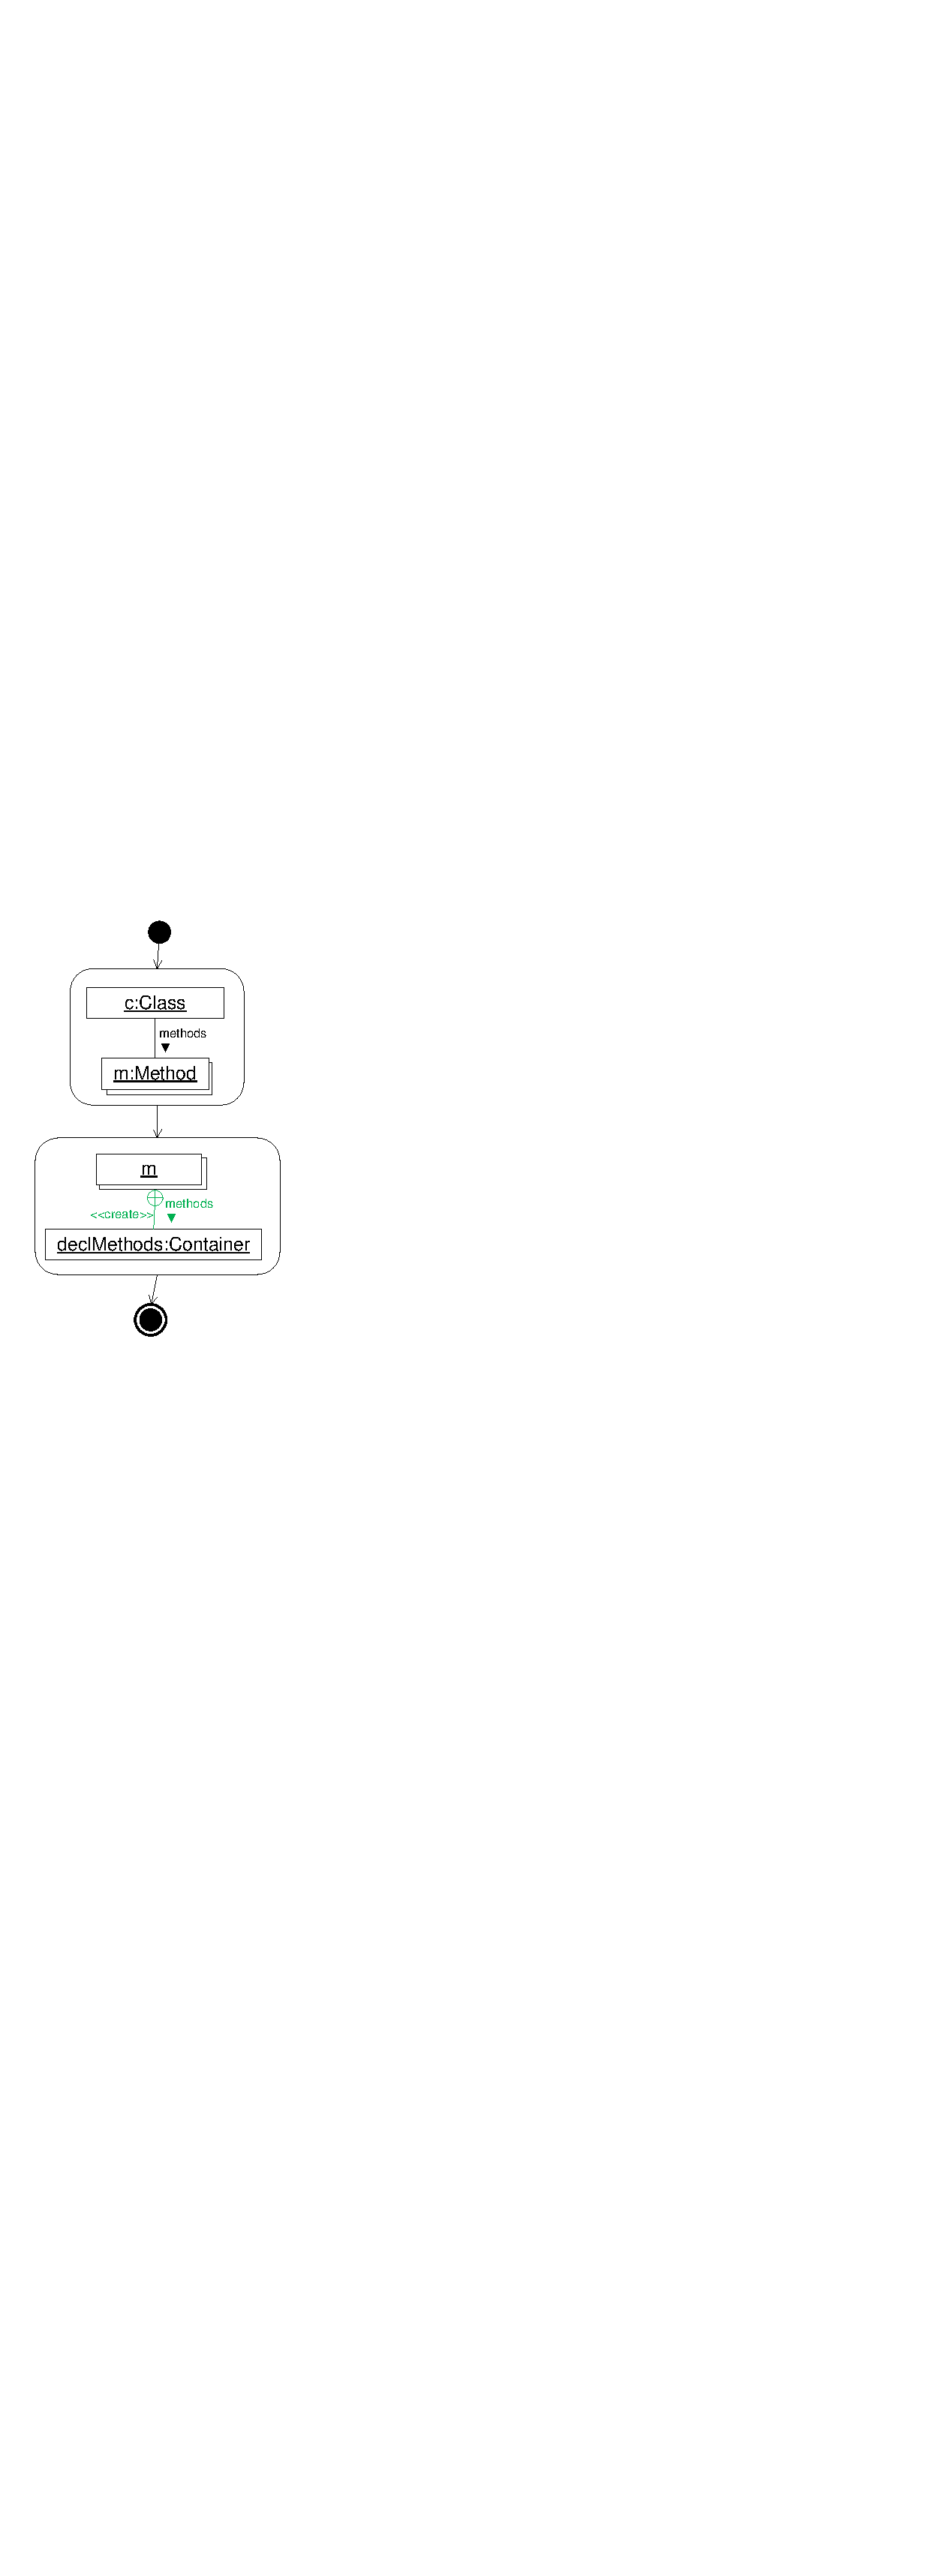
\includegraphics[scale=.8]{figures/ReuseObjectSet}
  	\caption{Reusing Object Sets}
  	\label{fig:reuseObjSet}
	\end{minipage}
  \hfill
  \begin{minipage}{.45\textwidth}
  	\centering
		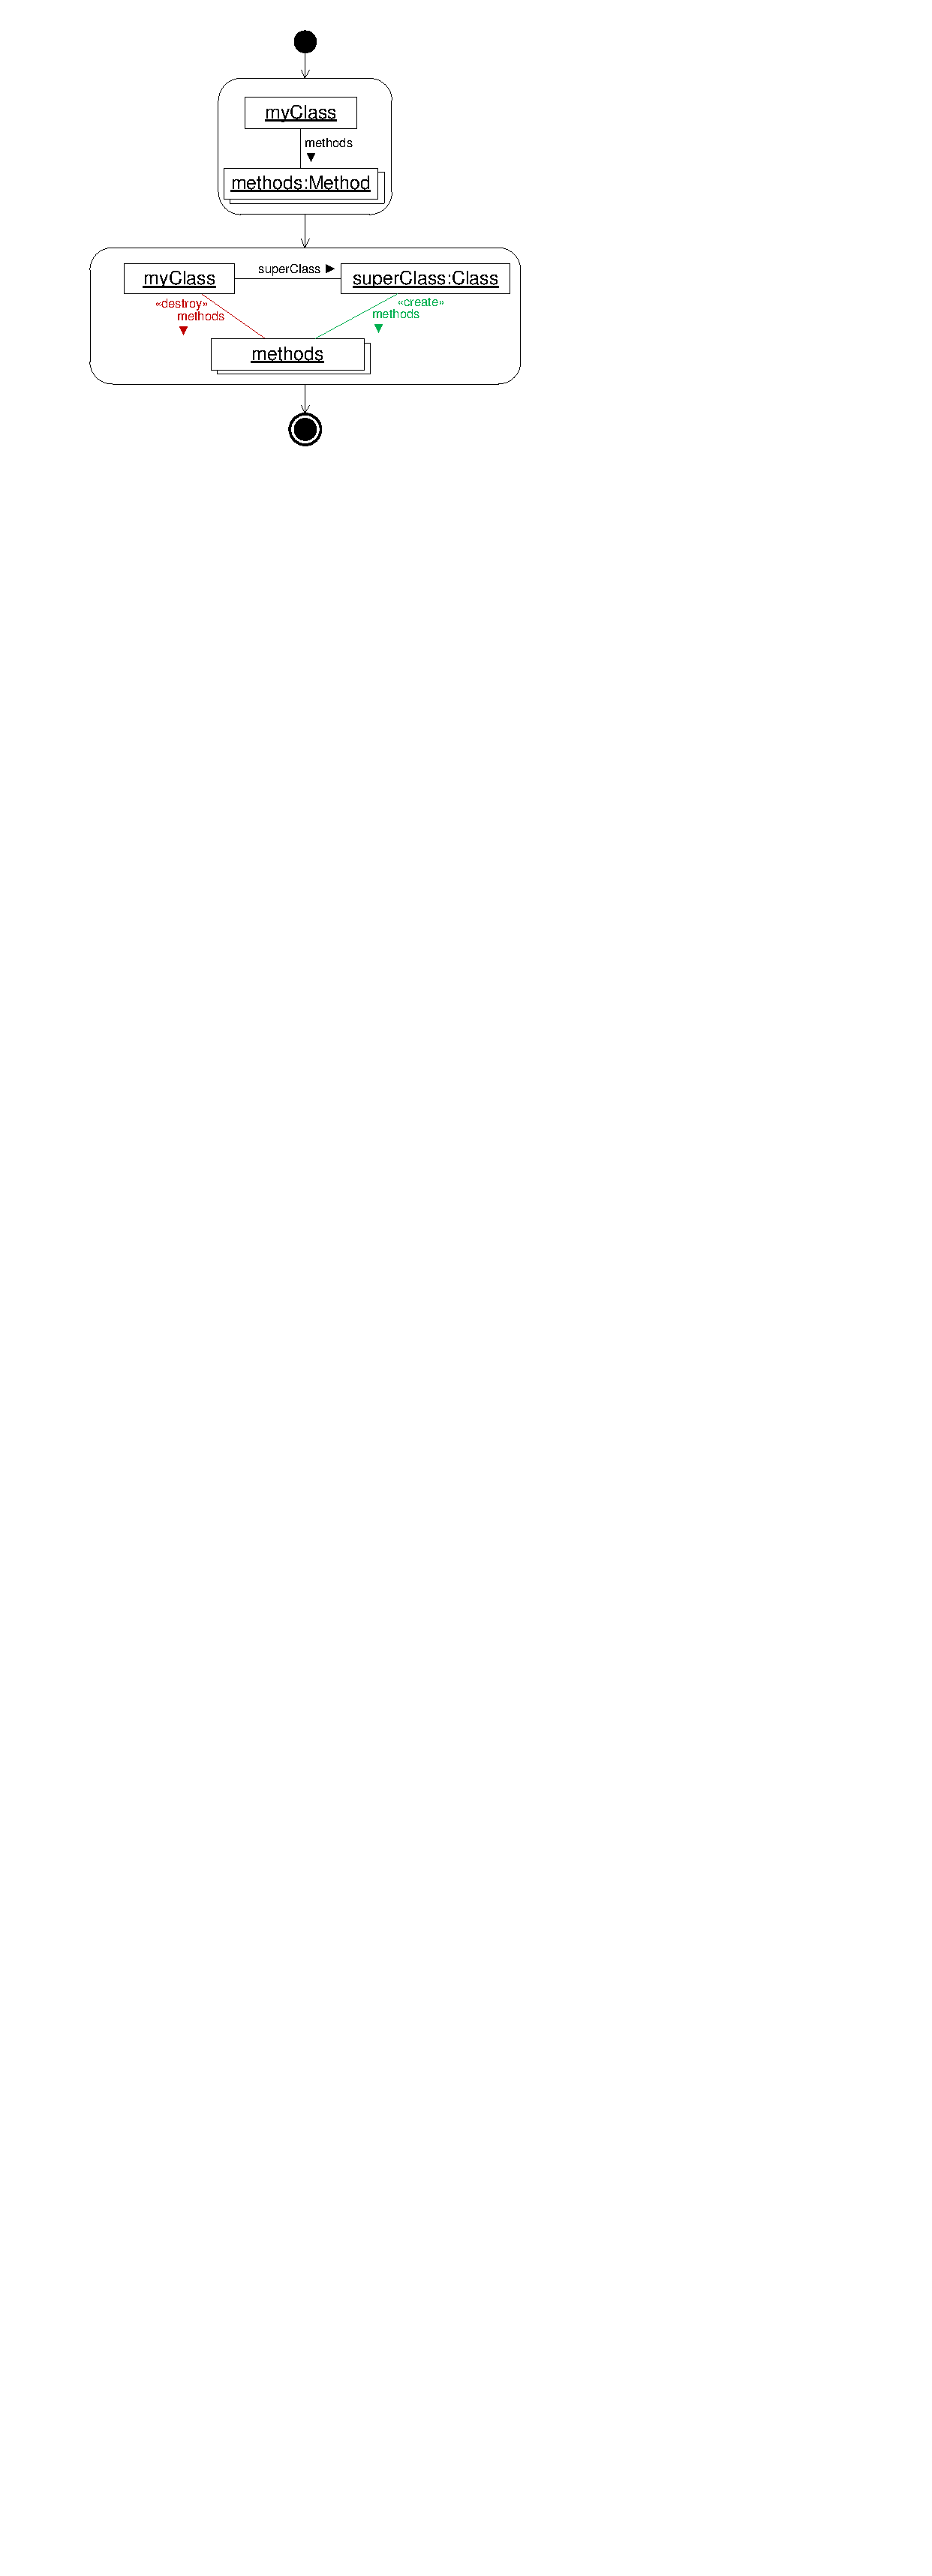
\includegraphics[scale=.8]{figures/ReuseObjectSet1}
  	\caption{Reuse objects in a set}
  	\label{fig:reuseObjSet1}
	\end{minipage}
\end{figure}

\begin{figure}[p]
	\begin{minipage}{.45\textwidth}
		\centering
		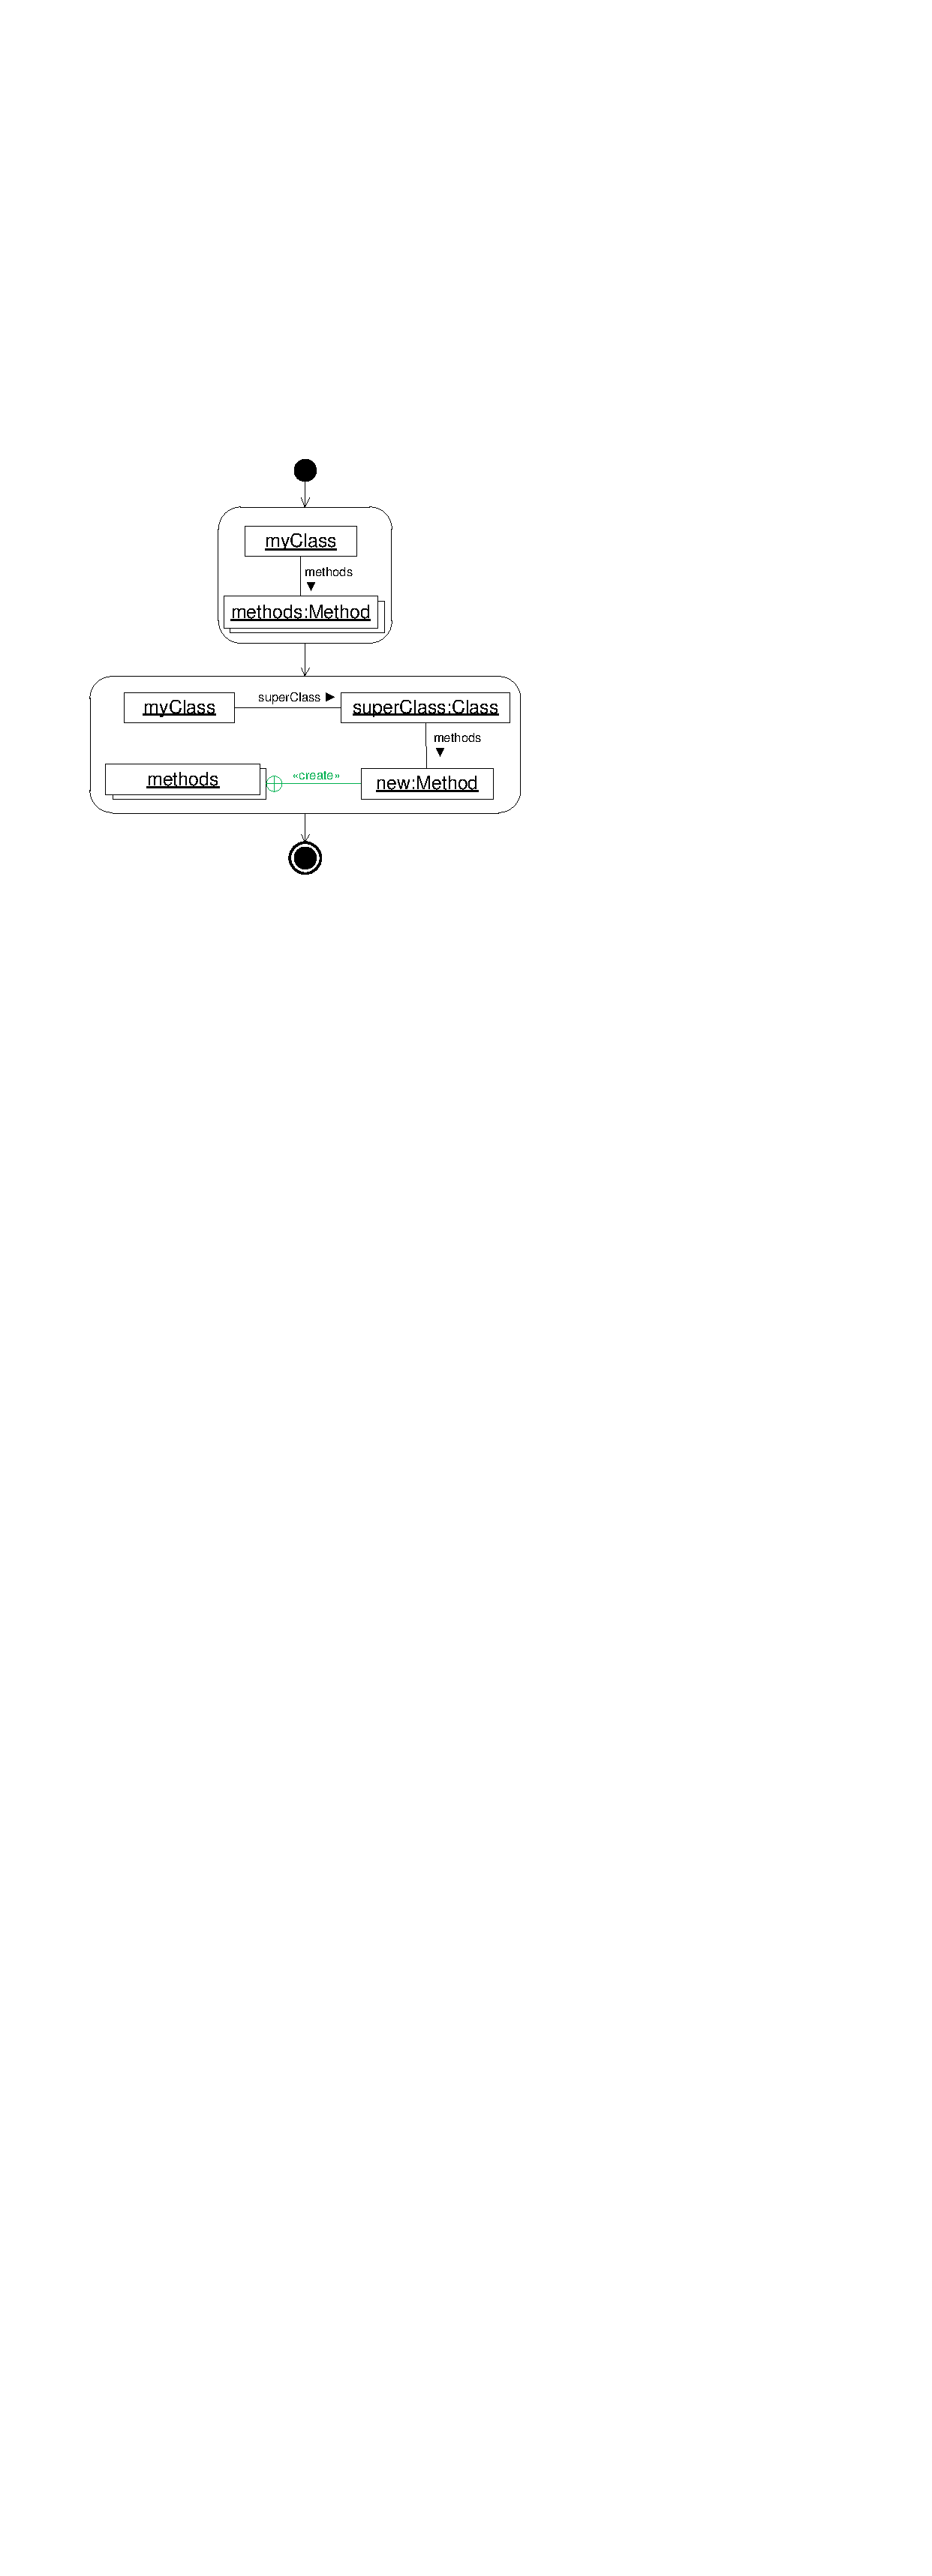
\includegraphics[scale=.8]{figures/ReuseObjectSet2}
  	\caption{Add an object to a set}
  	\label{fig:reuseObjSet2}
	\end{minipage}
  \hfill
  \begin{minipage}{.45\textwidth}
  	\centering
		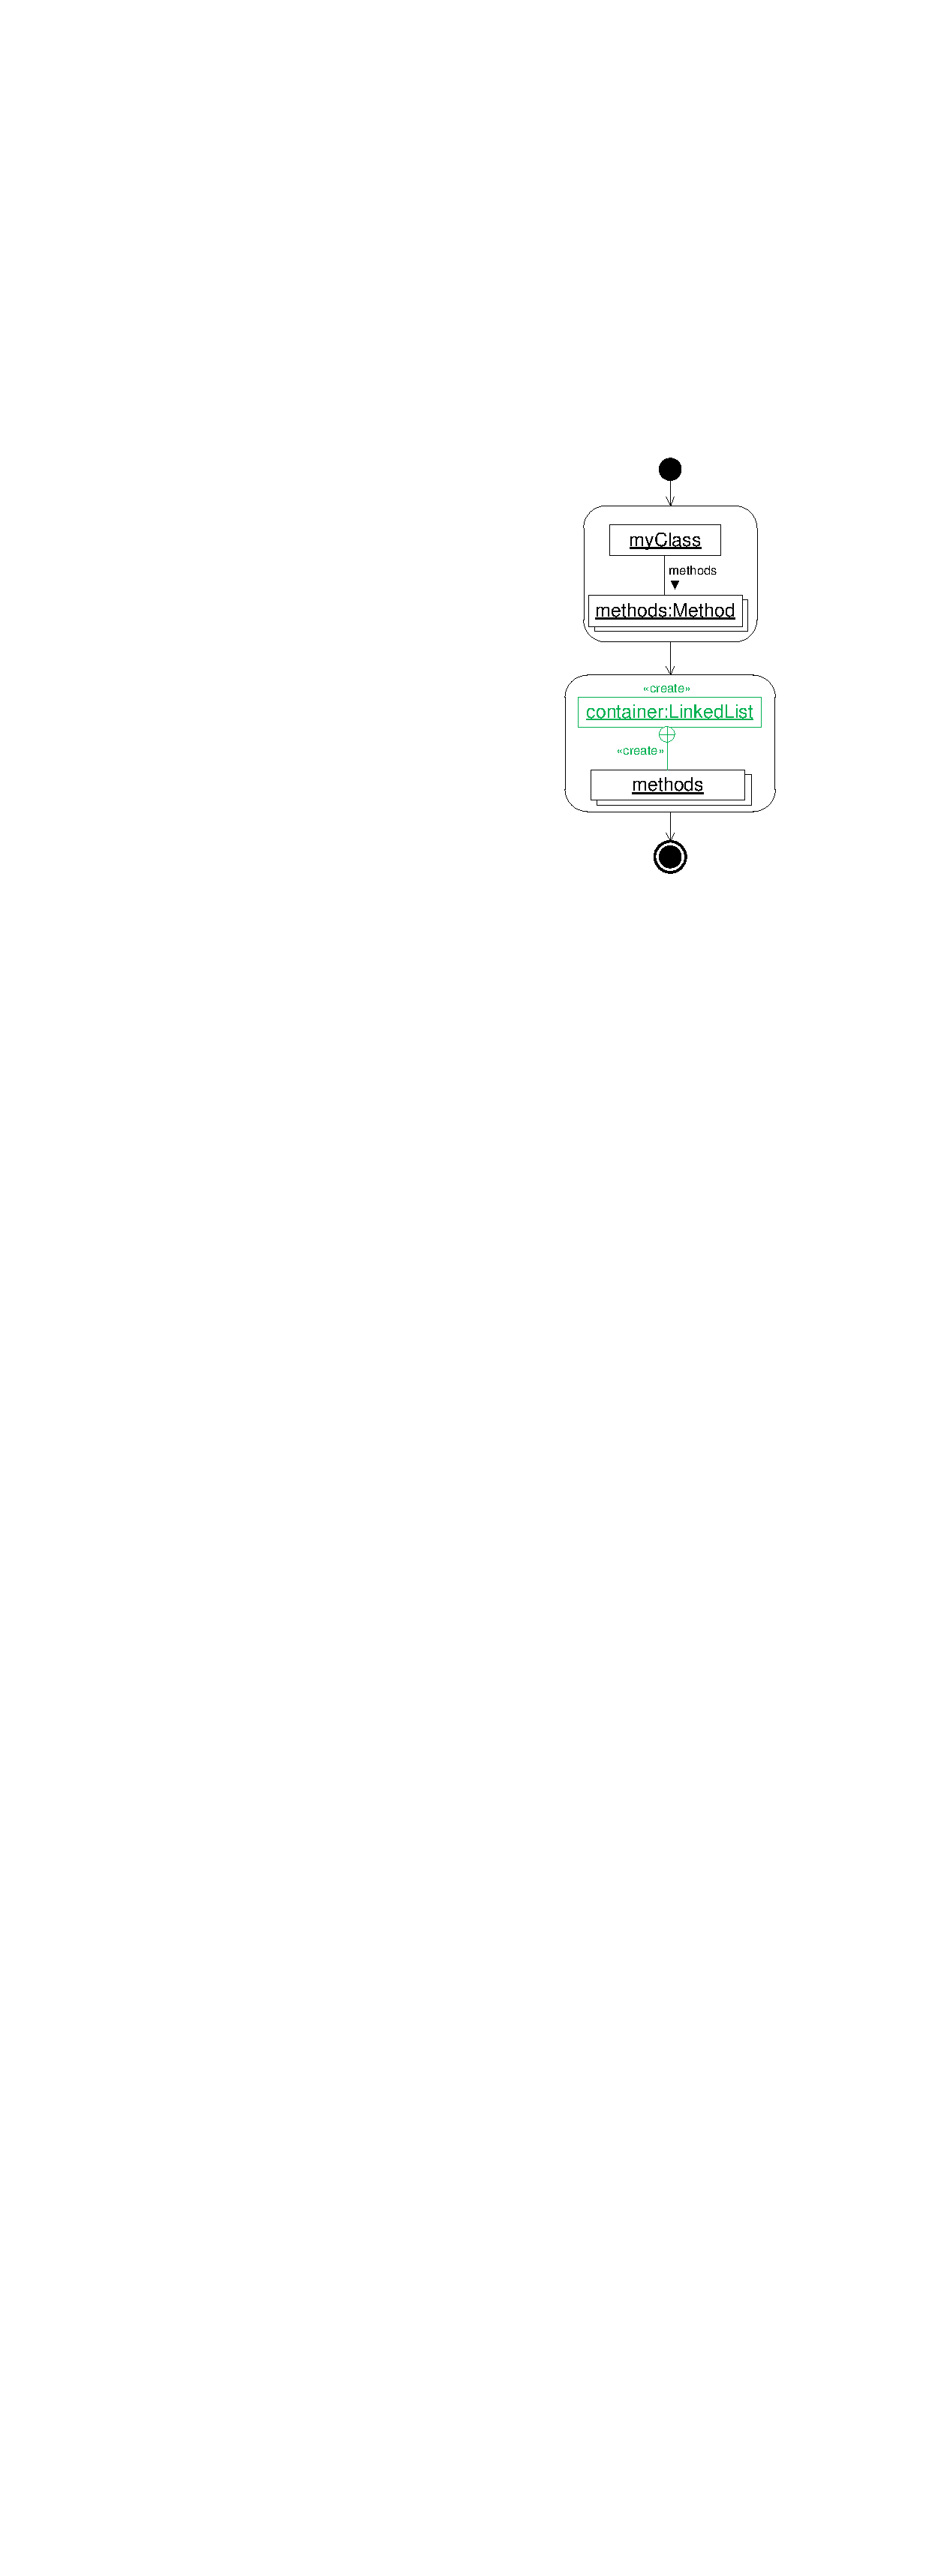
\includegraphics[scale=.8]{figures/ReuseObjectSet3}
  	\caption{Add all objects from a set to a container}
  	\label{fig:reuseObjSet3}
	\end{minipage}
\end{figure}

\todomcp{An object set contains no ObjectSetSizeExpression and no object is matched into the object set: ObjectSet is interpreted as optional and the matching succeeds.}

\todomcp{All operators for comparison are allowed: <, <=, >, >=, = !=}


\begin{figure}[p]
	\begin{minipage}{.45\textwidth}
		\centering
		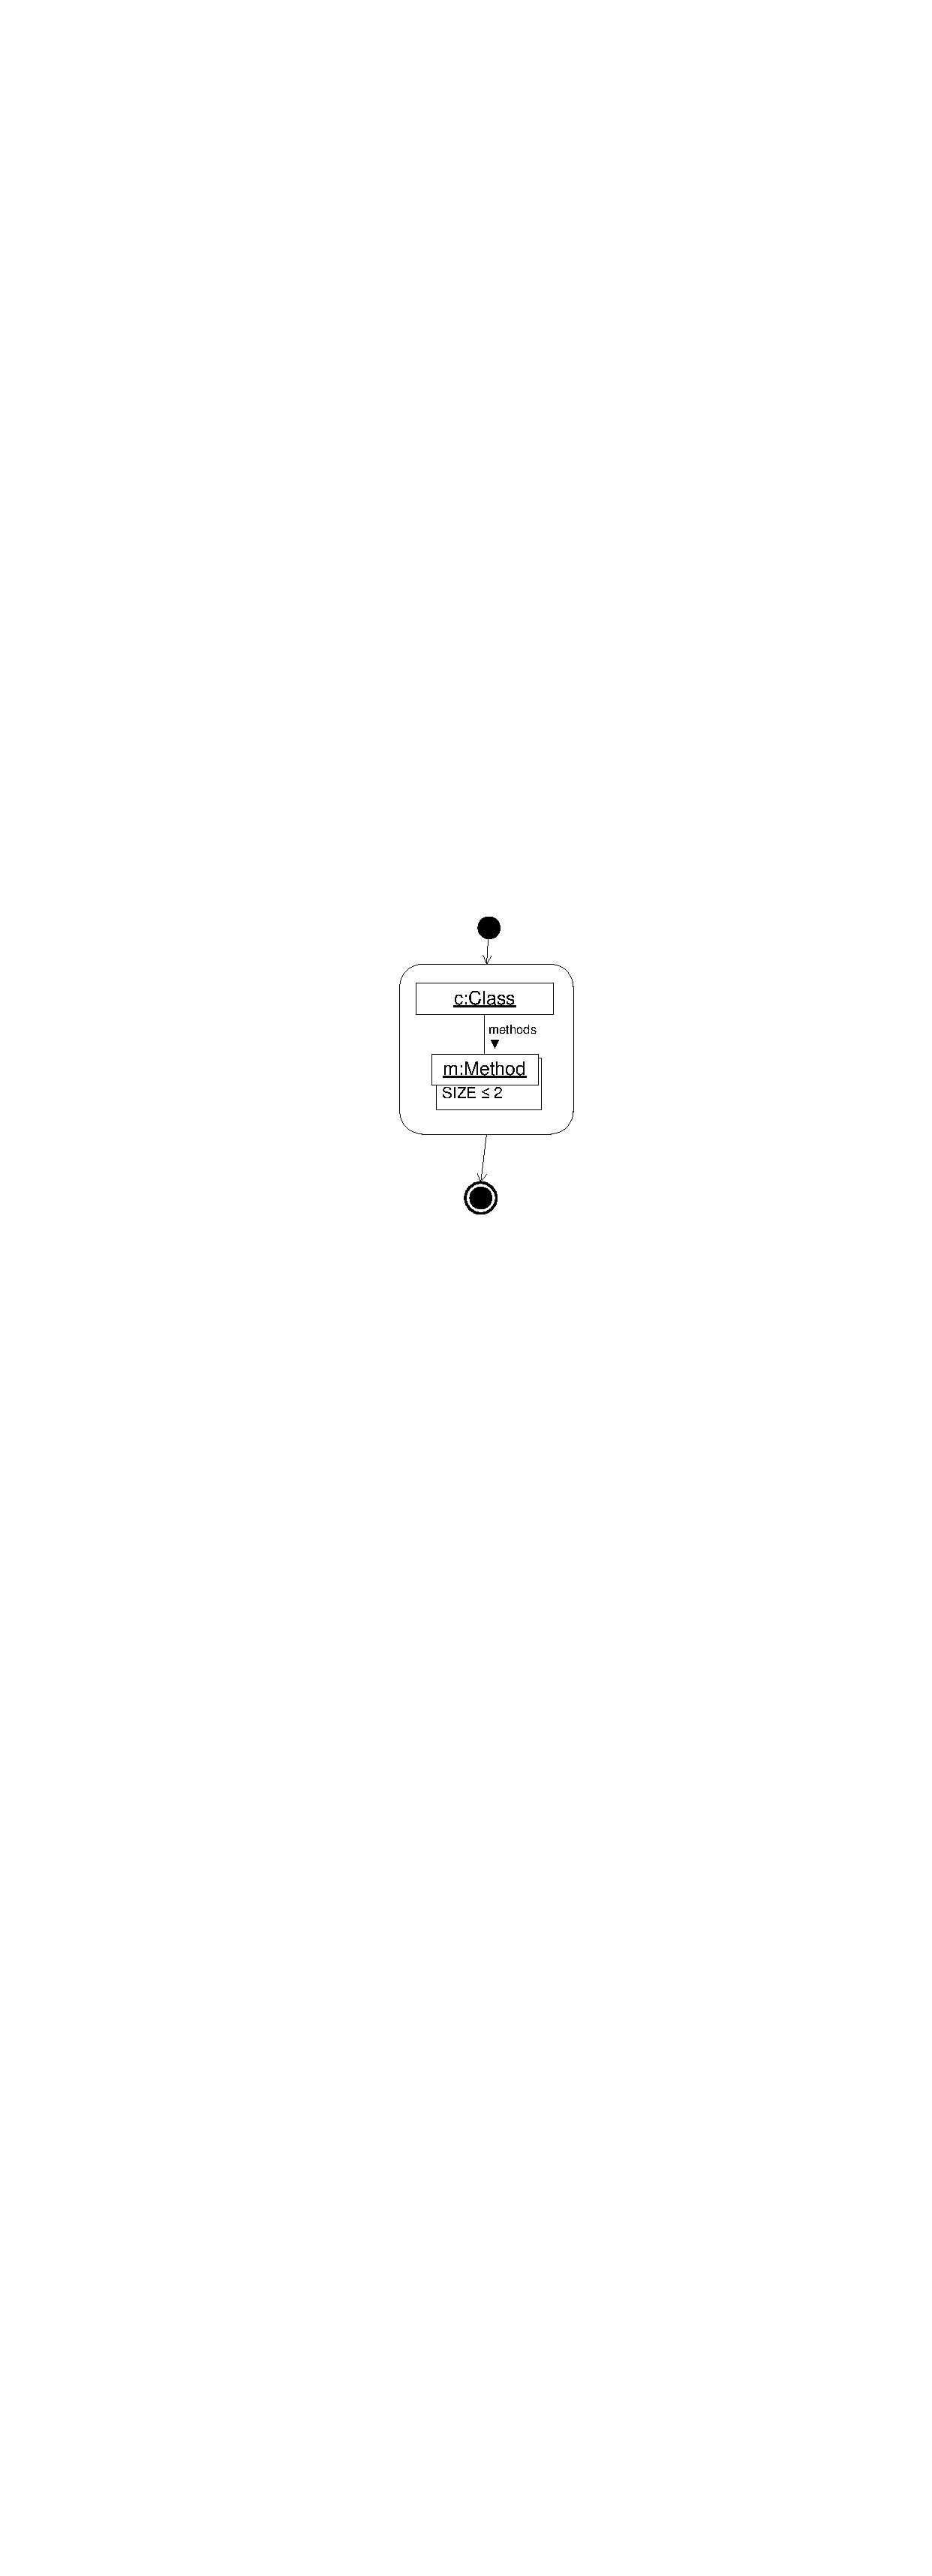
\includegraphics[scale=.8]{figures/ObjectSetSize}
  	\caption{Object Set Size}
  	\label{fig:objSetSize}
	\end{minipage}
  \hfill
  \begin{minipage}{.45\textwidth}
  	\centering
		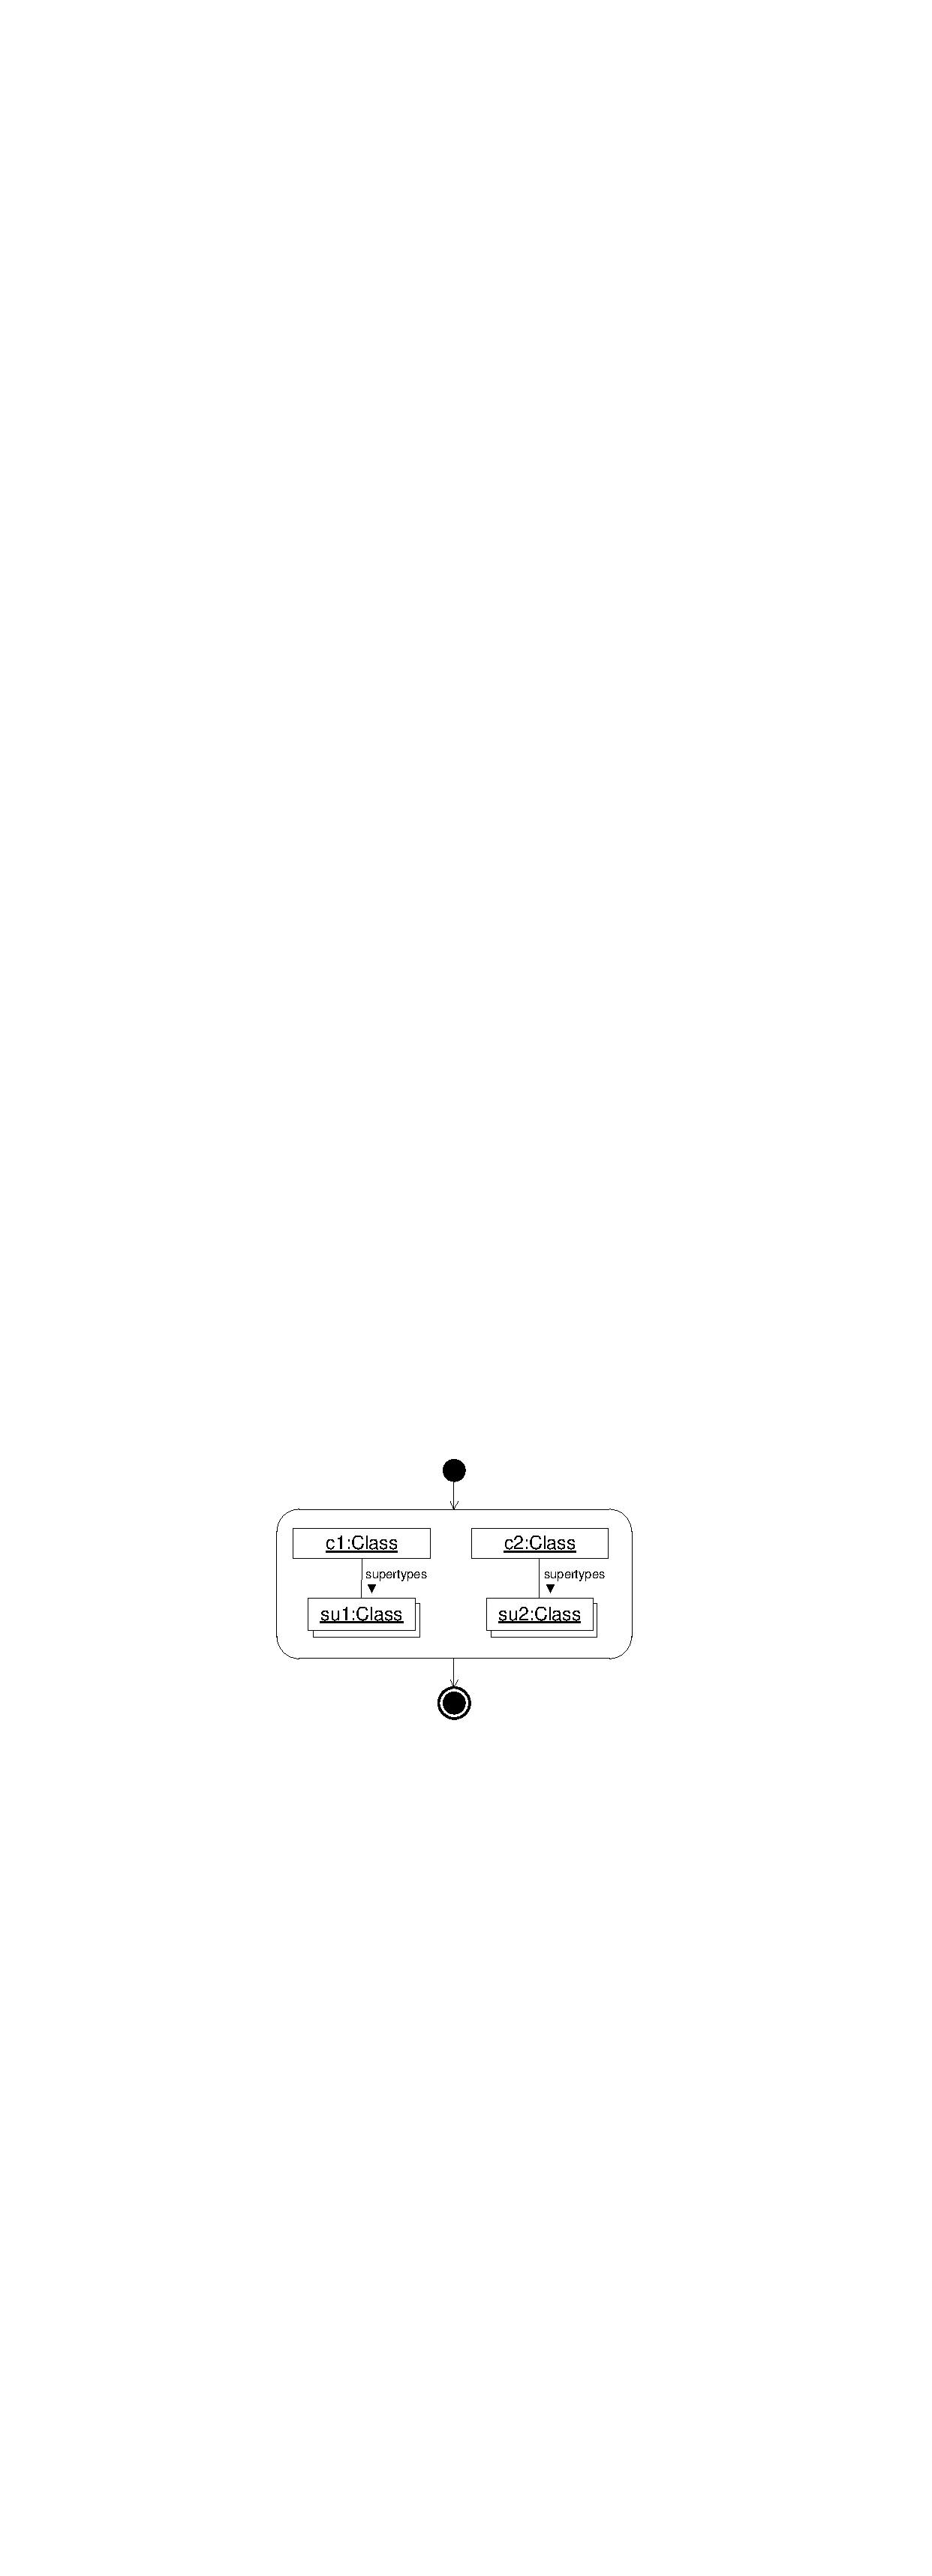
\includegraphics[scale=.8]{figures/IsomorphismInObjectSets}
  	\caption{Isomorphism in Object Sets}
  	\label{fig:isoObjSet}
	\end{minipage}
\end{figure}

\todomcp{What happens if one pattern contains two object sets that may possibly contain the same objects. Consider the pattern in Figure \ref{fig:isoObjSet}. If c1 and c2 share the same super classes, su1 and su2 contain the same objects. Is this allowed? Isomorphic matching would normally forbid this.}

\tododt{I would allow this which would comply with our isomorphic matching.
But in this case it is non-deterministic how the objects are matched to the set nodes (assuming the classes are already bound).
A maybe constraint could allow to match the same objects to both sets.}
\todojr{We decided to match set nodes without them having to be disjoint, thus, we do not enforce isomorphism for the content of two or more set variables.}
}%------ End of object set section




\ext  %--- Comment this line to include special link kinds into the document
{
\subsection{Special Link Kinds [CH]}
\label{sec:StoryPatterns:specialLinks}

\subsubsection{Inclusion Links [CH]}
\label{sec:StoryPatterns:specialLinks:inclusion}

\todoch{What is the semantics of a containment link? Current understanding: an element is contained in a container. What is the difference to to-many references which are containments?}
\tododt{Containment links do not correspond to any association or reference. They only describe containments of objects in containers or set nodes.}

\todoch{Which classifiers are allowed for ContainerVariables? This should not only be the EMF collection types EList and EMap. Does a ContainmentLink need a reference as a type like normal LinkVariables?}
\tododt{The contaiment links do not need any reference. I would suggest to allow any subtype of java.util.Collection (and java.util.List in case that link order constraints are used), but not java.util.Map! This is something different and needs a key for containment. Maybe we need special containment links for maps that include a key.}

\subsubsection{Paths [MCP]}
\label{sec:StoryPatterns:specialLinks:paths}

\subsubsection{Link Constraints [CH]}
\label{sec:StoryPatterns:specialLinks:linkConstraints}

\todoch{What is the concrete Syntax for this?}

\tododt{I have a suggestion in Figure~\ref{fig:linkConstraints}.}

\begin{figure}[p]
  \centering
  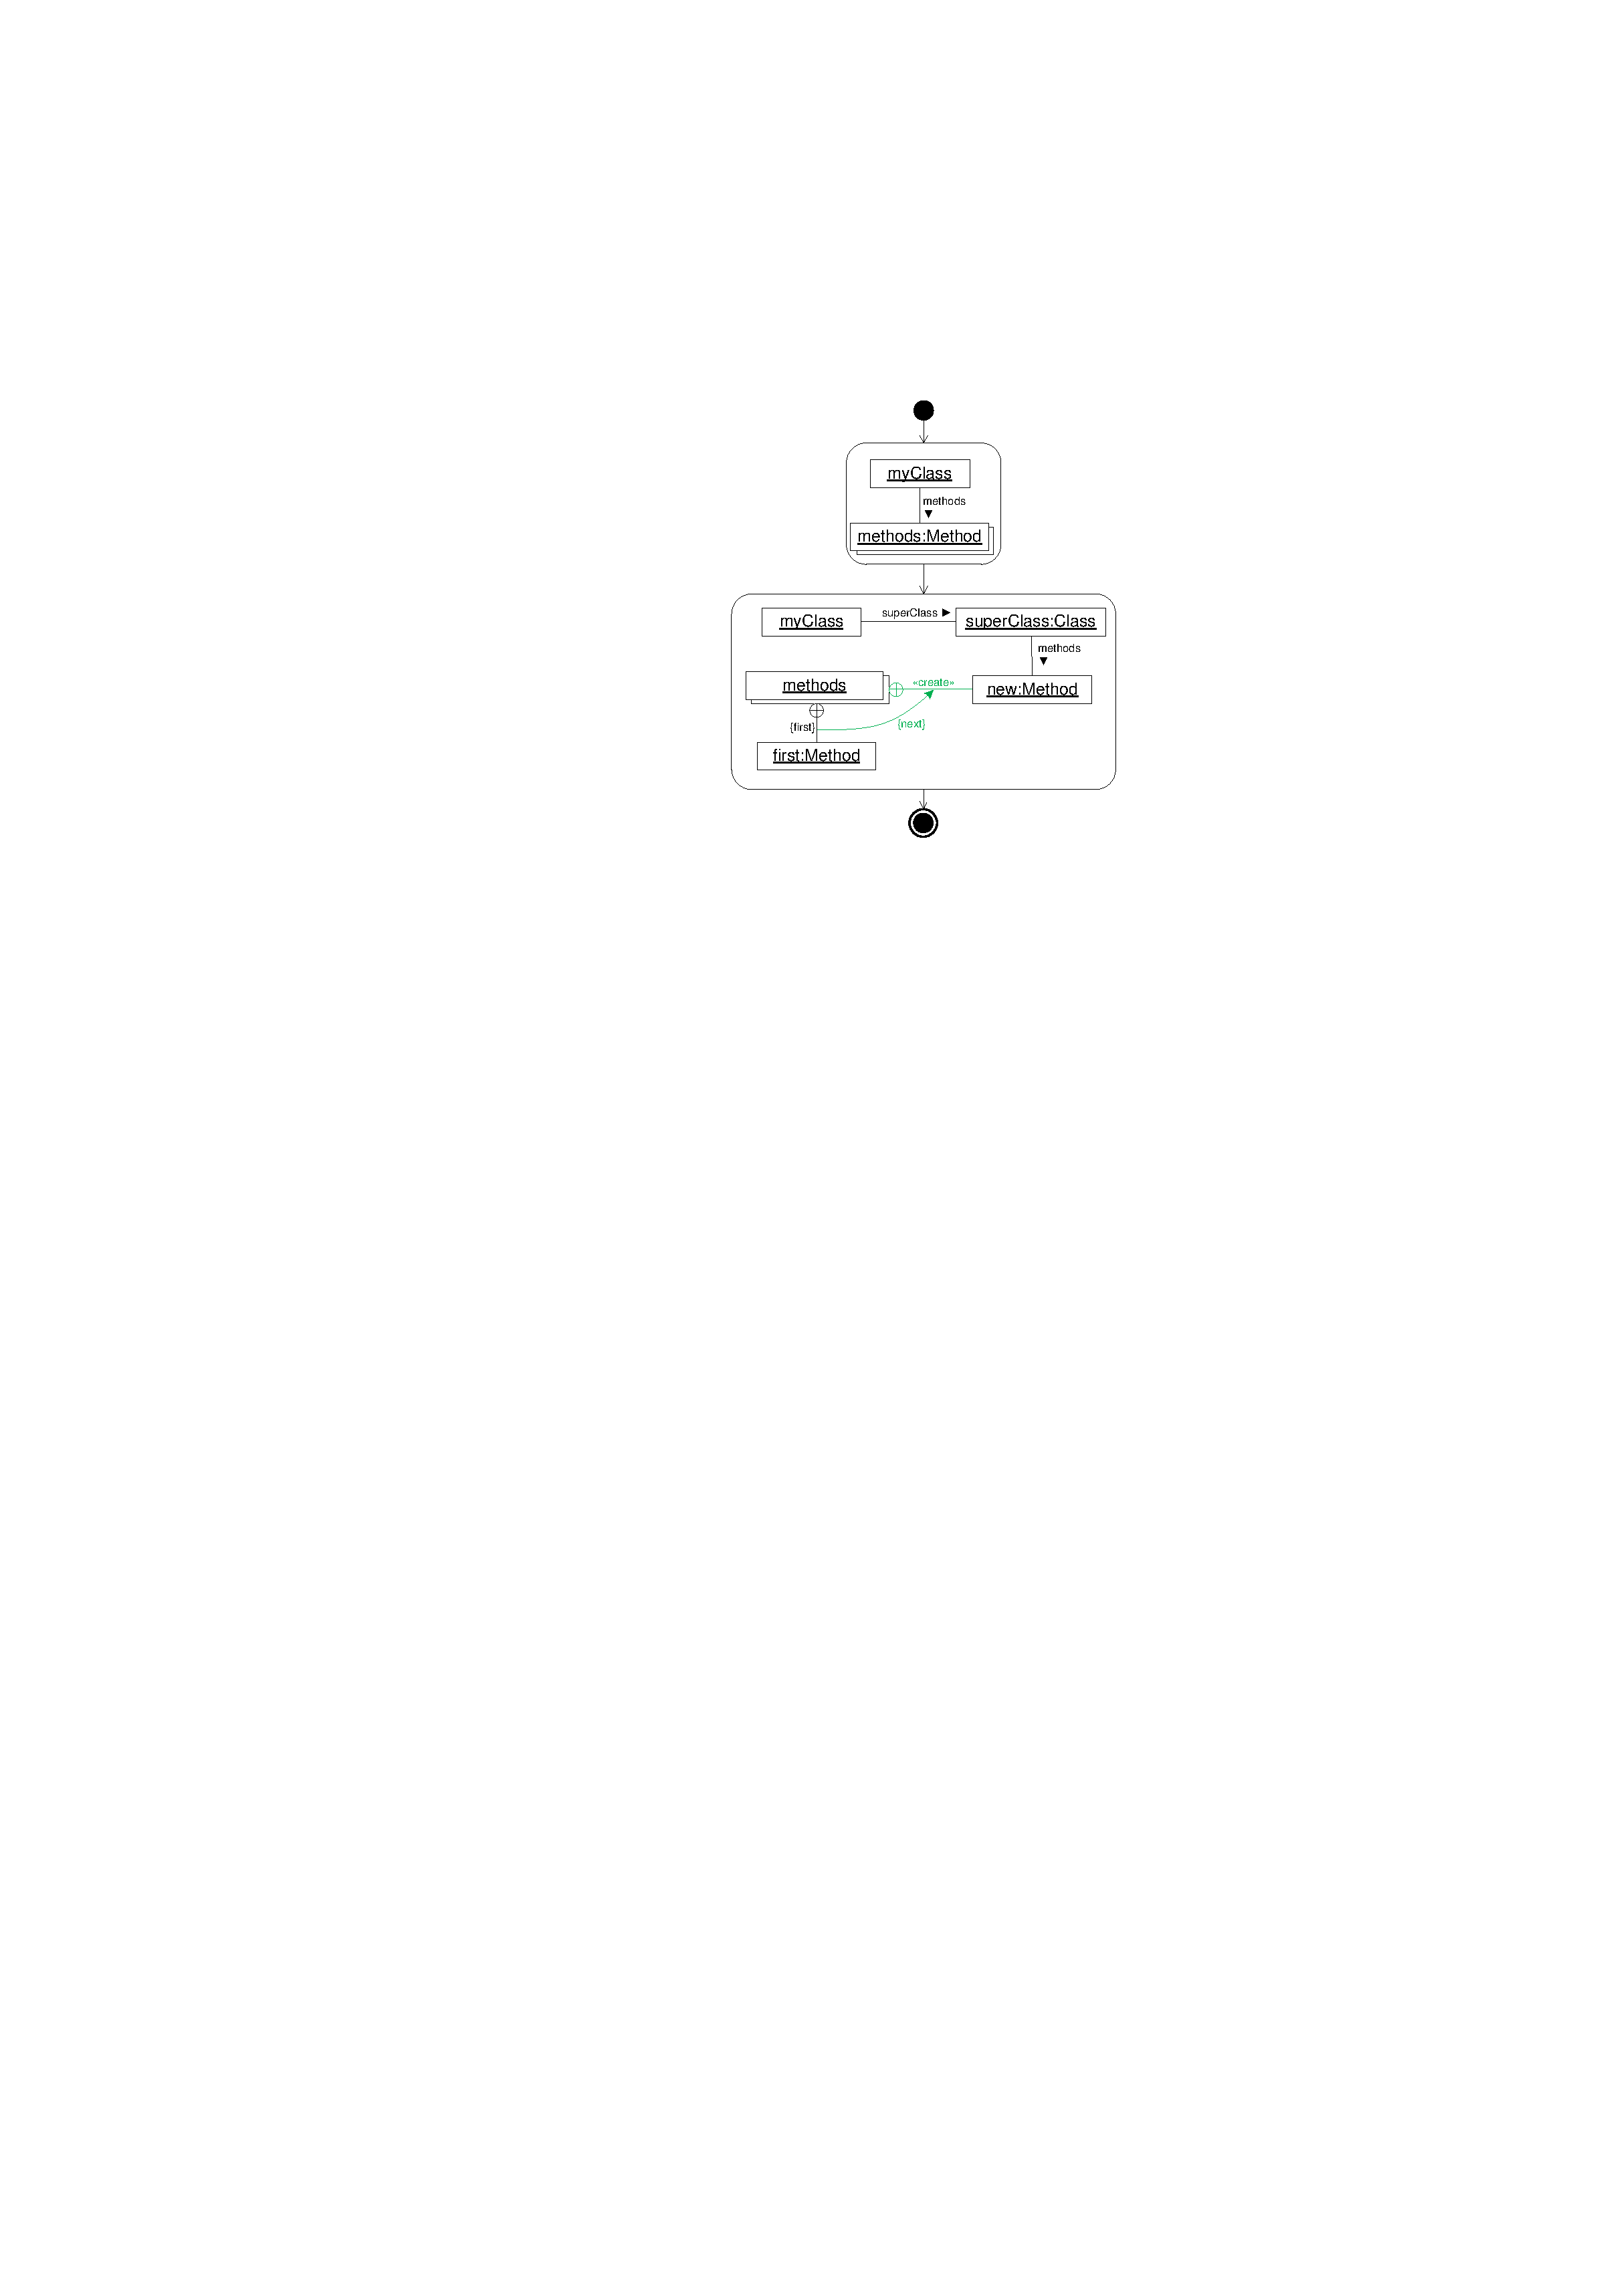
\includegraphics[scale=.8]{figures/LinkConstraints1}
  \caption{Link order constraints FIRST and DIRECT\_SUCCESSOR}
  \label{fig:linkConstraints}
\end{figure}

Link constraints are only applicable to link variables that reference an ordered to-many reference.
\todoch{No link constraints for inclusion links.}

\begin{itemize}
  \item FIRST = matches the first element in the list, requires one link variable
  \item LAST = matches the last element in the list, requires one link variable
%  \item INDEX = matches the element at the specified index, requires one link variable
%  \todoch{Our lowest index value is 0, not 1.}
  \item DIRECT\_SUCCESSOR = requires two link variables, target of the second one must be located directly after the target of the first one in the list
  \item SUCCESSOR = requires two link variables, target of the second one must be located somewhere after the target of the first one in the list
\end{itemize}

\todojr{We will separate link constraints for single links and those for two links and their order. Stephan will make a suggestion.}

\todoch{Is this semantic description correct/complete?}

\todoall{Stephan: Following is my suggestion for link constraints.}

Link constraints specify constraints on the absolute position of an element in an ordered reference and the position of an element relative to another element. These constraints are only applicable to \emph{LinkVariables} that refer to ordered multi-valued references. Other kinds of links cannot be adorned with link constraints.

\paragraph{Link Position Constraints}

\begin{figure}[htb]
\center
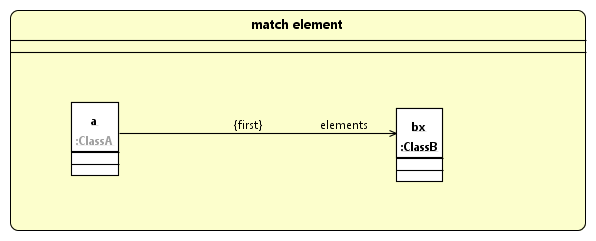
\includegraphics[width=0.75\columnwidth]{figures/linkPositionConstraint1.png}
\caption{A \emph{first} link position constraint}
\label{fig:linkPositionConstraints:linkPositionConstraint1}
\end{figure}

A link position constraint specifies that the target object of the constrained link has to be the \emph{first} or the \emph{last} element in that reference. For example, in a valid match of the story pattern in Fig.~\ref{fig:linkPositionConstraints:linkPositionConstraint1}, the object matched to \emph{bx} must be also be the first element in the \emph{elements} reference of the object matched to \emph{a}. Link position constraints support only these two positions: \emph{First} and \emph{last}. If a story pattern contains multiple links that refer to the same metamodel reference and have the same source variable, only one of them may have a \emph{first} (or \emph{last}) constraint.

When link position constraints are attached to links with \destroy stereotypes, the semantics are identical, even if they are optional. For links with \create stereotype, the link's target element is inserted at the specified position. For optionally created links, the semantics is somewhat different. If the link does not yet exist, it is created. The target element is inserted at the specified position in the reference. If the link does exist but the element is not at the specified position, it is moved.

\todoall{Alternatives: 1. Ignore link position constraints on optional-create links, 2. add target element a second time. For unique references, this has the same effect like moving the element, in case of non-unique references, the element exists twice (or more times) in the list, afterwards.}

\begin{figure}[htb]
\center
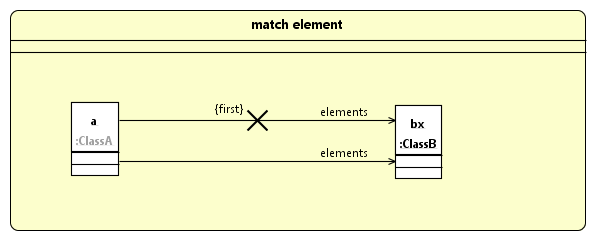
\includegraphics[width=0.75\columnwidth]{figures/linkPositionConstraint2.png}
\caption{A negative link position constraint}
\label{fig:linkPositionConstraints:linkPositionConstraint2}
\end{figure}

A combination with negative links is also straight-forward. In a valid match of the pattern shown in Fig.~\ref{fig:linkPositionConstraints:linkPositionConstraint2}, the match of \emph{bx} must \emph{not} be the first element in the \emph{elements} reference.

\paragraph{Link Order Constraints}

\begin{figure}
\center
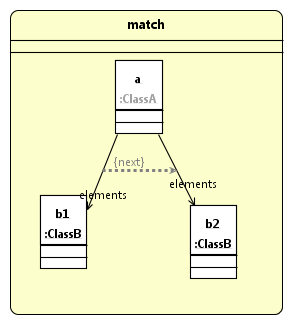
\includegraphics[width=0.4\columnwidth]{figures/linkOrderConstraint1.png}
\caption{A link order constraint specifies a relative order between two links.}
\label{fig:linkOrderConstraints:linkOrderConstaint1}
\end{figure}

Link order constraints specify a relative order between two links. In Fig.~\ref{fig:linkOrderConstraints:linkOrderConstaint1}, \emph{b2} must be the immediate successor of \emph{b1} in the \emph{elements} reference (depicted by \emph{\{next\}}). It is also possible to specify that \emph{b2} may be a direct or indirect successor, which is depicted by \emph{\{...\}}. Note, that then there may be multiple possible matches. Which of them is chosen is still non-deterministic.

Link order constraints can be combined straight-forwardly with \create and \destroy stereotypes. However, the combination with \create is only possible for the \emph{\{next\}} order constraint, not for \emph{\{...\}}. In case of created links, the order in the instance model is enforced accordingly.

\todoall{Do we want to allow this? This would make the choice, where an element is inserted non-deterministic.}

It is also possible to have only one of the two related links be destroyed or created. Though, it is not possible to create one link and destroy the other.

Link order constraints may not form circles or unsatisfiable story patterns (e.g., where a link is the successor of another but also has a \emph{\{first\}} link position constraint).

\begin{figure}
\center
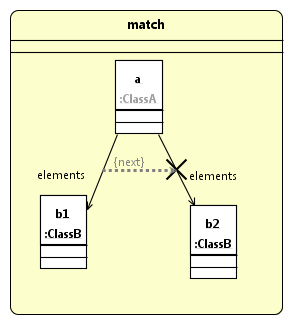
\includegraphics[width=0.4\columnwidth]{figures/linkOrderConstraint2.png}
\caption{A link order constraint with a negative link.}
\label{fig:linkOrderConstraints:linkOrderConstaint2}
\end{figure}

Link order constraints can also be combined with negative link. However, only one of both links may be marked as negative. Otherwise, there would be nothing to relate to. For example, in the story pattern in Fig.~\ref{fig:linkOrderConstraints:linkOrderConstaint2}, \emph{b2} may not be the direct successor of \emph{b1}.

\begin{figure}
\center
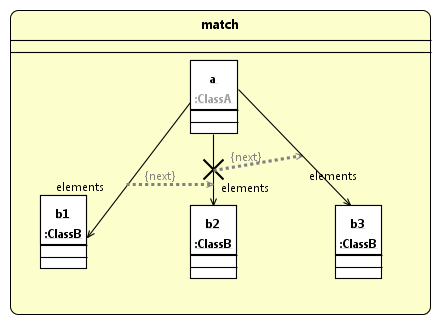
\includegraphics[width=0.6\columnwidth]{figures/linkOrderConstraint3.png}
\caption{Two link order constraints with a negative link.}
\label{fig:linkOrderConstraints:linkOrderConstaint3}
\end{figure}

If there are multiple link order constraints, like in Fig.~\ref{fig:linkOrderConstraints:linkOrderConstaint3}, the semantics of the negative link is as follows: \emph{b2} must neither be the direct successor of \emph{b1} nor the direct predecessor of \emph{b3}. If one of both conditions is fulfilled, the pattern does not match.

\todoall{This should match the semantics of multiple NACs in a story pattern.}

For optionally created and destroyed links, the same applies to link order constraints like to link position constraints. Optionally destroyed link can be used straight-forwardly. An optionally created link is created if it does not exist, so that the specified order is enforced. If the link does exist but the element is not at an appropriate position, it is moved.

\subsubsection{Maybe Links}
\label{sec:StoryPatterns:specialLinks:maybeLink}

Story pattern are matched by using isomorphic matchings. That means that two object variables in a story pattern may not be matched to the same object of the instance model. A matching which matches two object variables to the same object is, thus, considered to be invalid. In some situations, however, such matchings should be explicitly allowed. Then, the isomorphic matching must be disabled. This may be achieved by connecting the object variables with a maybe link. Figure \ref{fig:maybeLink} shows the concrete syntax of maybe links. 

\begin{figure}[htbp]
  \centering
  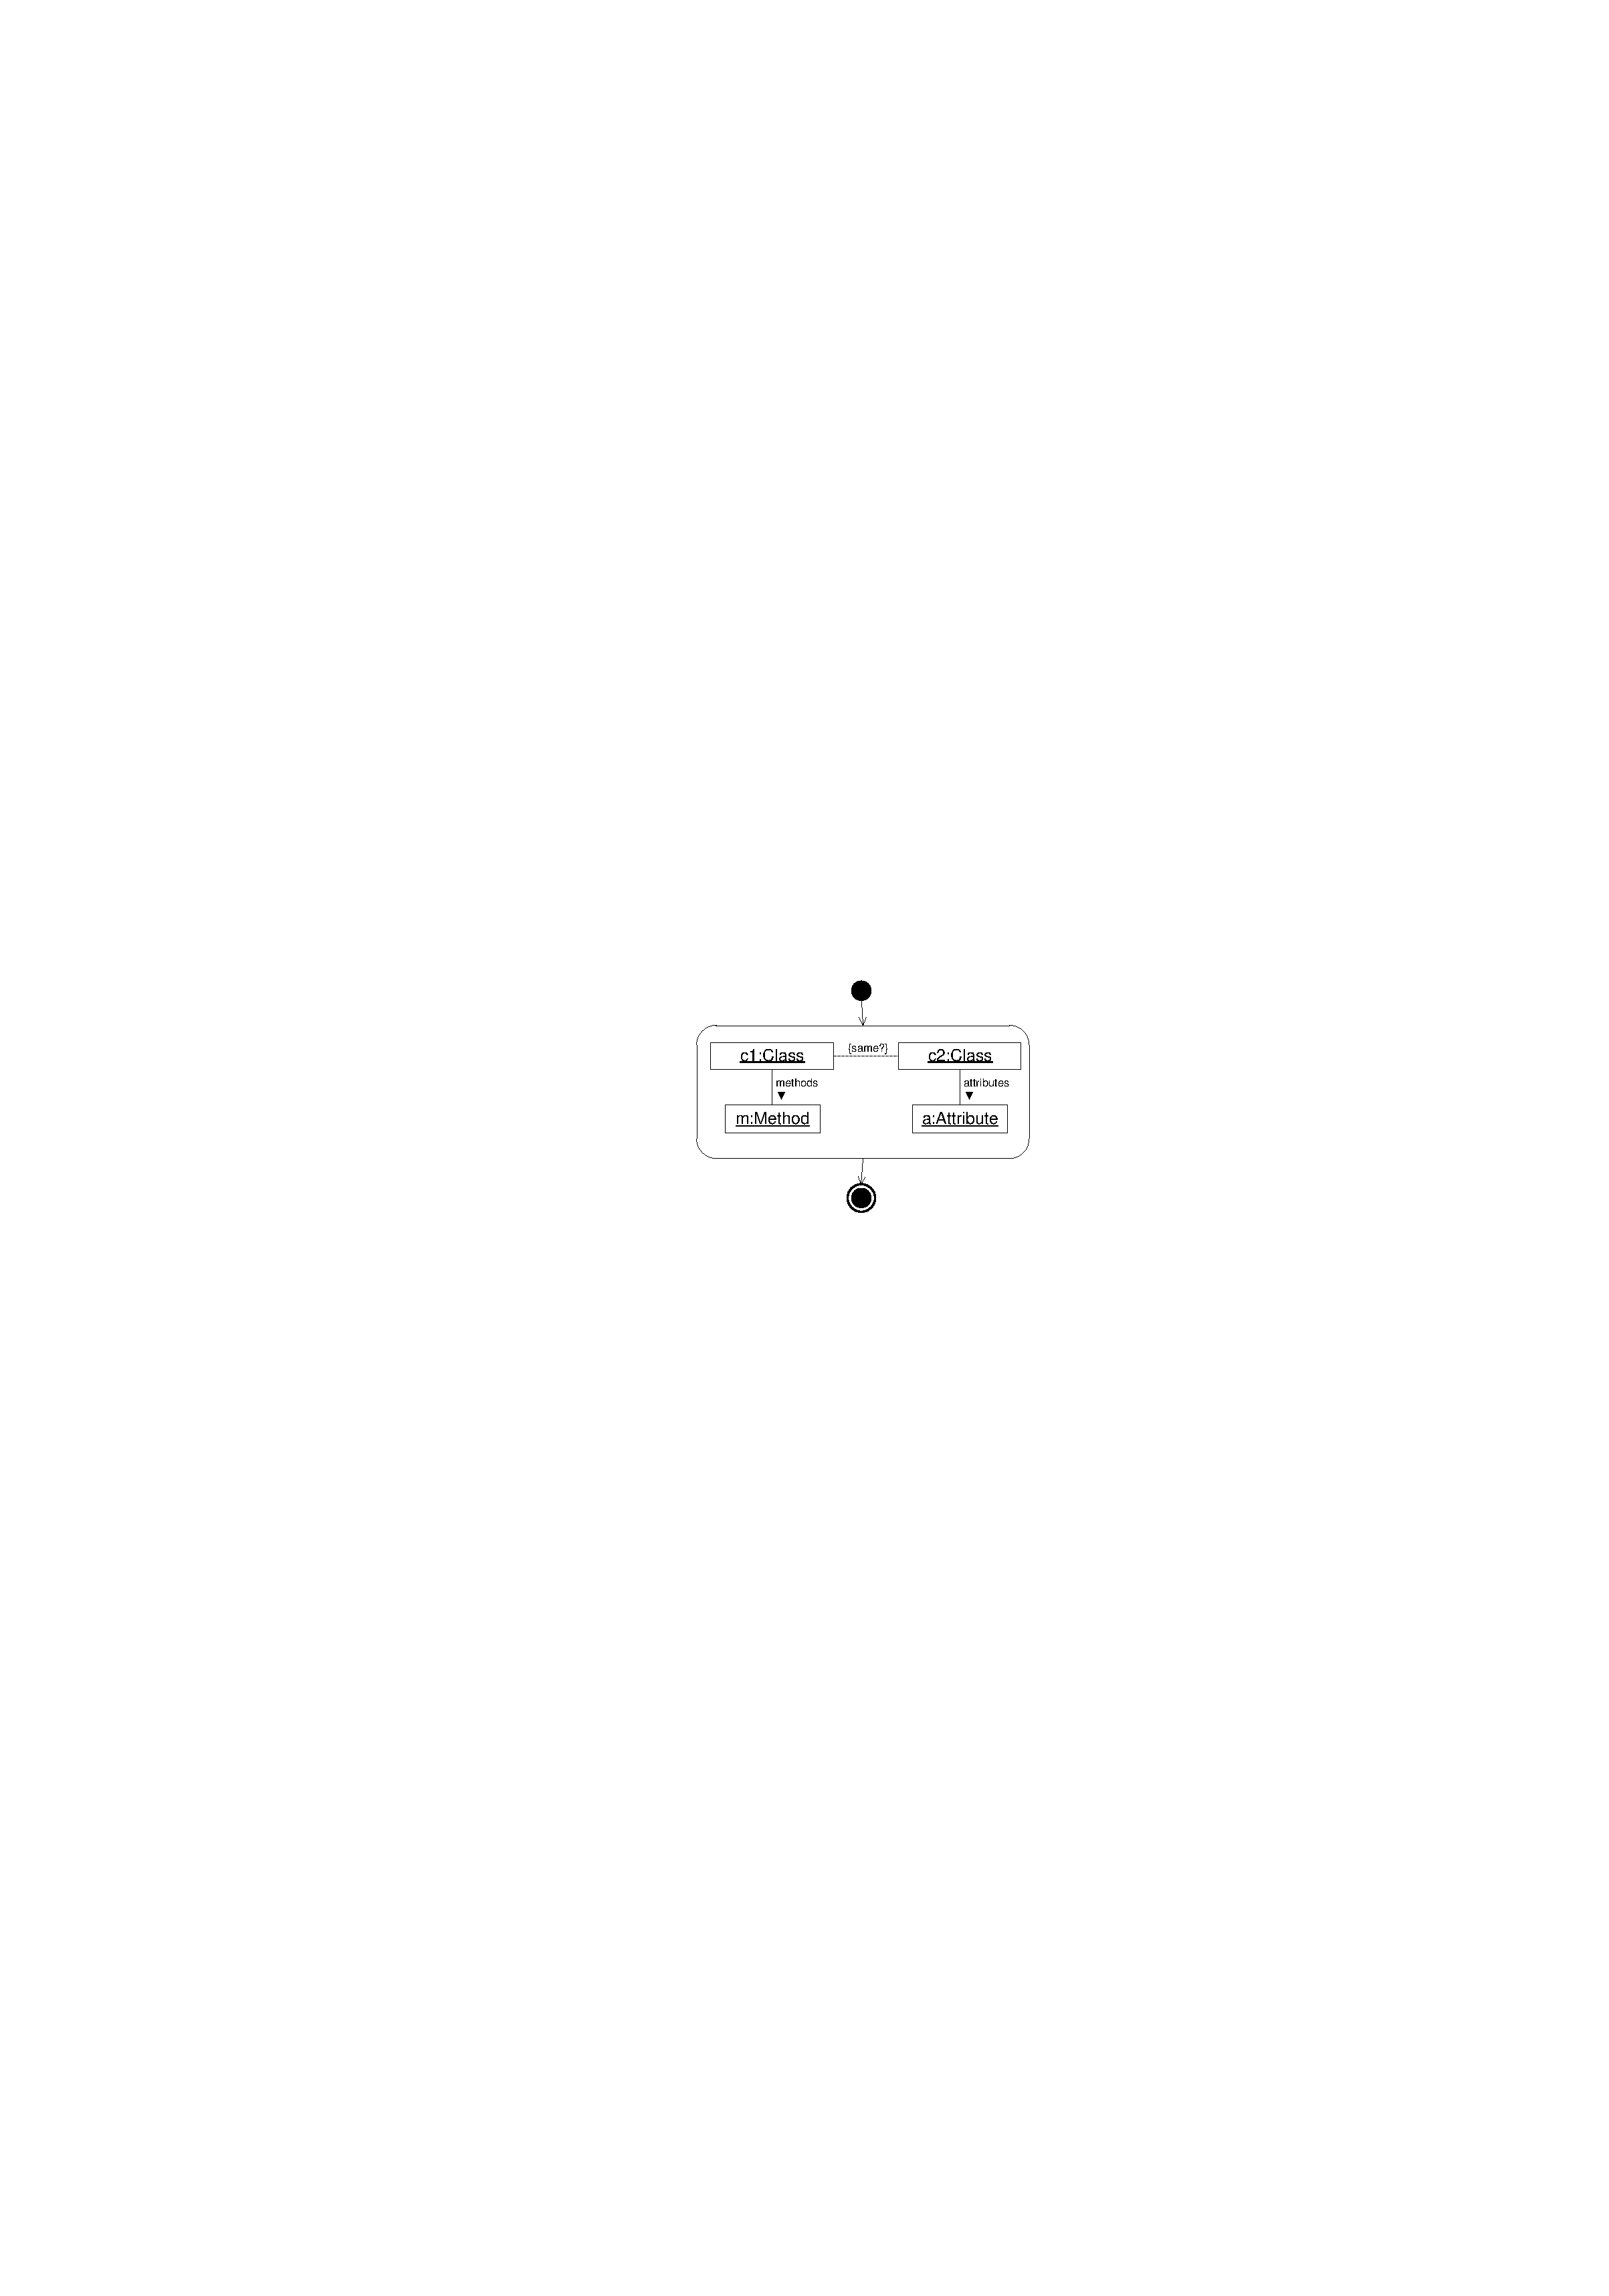
\includegraphics[scale=.8]{figures/MaybeLink}
  \caption{Maybe Link allowing two Object Variables to be matched to the same Object}
  \label{fig:maybeLink}
\end{figure}

If two object variables are connected by a maybe link, they both must be mandatory or optional. In addition, a maybe link requires the object variables to be matched or destroyed, but not created.  
} %--- End of special link kinds section



\ext  %--- Comment this line to include pattern constraints into the document
{
\subsection{Pattern Constraints [CH]}

\todoch{What happens when a pattern constraint is placed inside a for each story pattern (not inside a node in that pattern)? Proposal: The particular match must fulfill the pattern constraint, if it does not fulfill the pattern constraint, the match is rejected and the iteration continues.}
\tododt{Exactly. In this case, it is a kind of post condition that has to be satisfied at the end of the matching step.}

} %--- End of pattern constraints section




\ext  %--- Comment this line to include pattern fragments into the document
{
\subsection{Pattern Fragments [MCP]}

patterns contained in other patterns, negative, semantics? review enhanced story patterns from Diss Florian Klein

\todomcp{Should contained pattern be marked as forEach? Idea for semantics: first the part of the pattern outside the forEach pattern is matched, then the forEach subpattern is applied to any match that may be located, the variables bound in a forEach subpattern may not be used in subsequent activities}

\todoch{The transformations diagrams that Matthias Meyer developed in his Diss contain so-called iterated parts that are essentially the same as a for-each fragment. We should check his semantics.}

\tododt{This is somewhat confusing.
As I understand them, subpatterns are ordinary story patterns within another story pattern.
They are surrounded by a fragment box and can be labeled with a name (see Figure~\ref{fig:labeledSubPattern}).
Special types of such subpatterns are negative application condition fragments (NACs), set fragments, and optional fragments.
As far as I know, we did not plan to add $\forall$ and $\exists$ fragments, did we?
These are only used in SDDs and TSSDs which are constraint languages.
}

\begin{figure}[htbp]
  \centering
  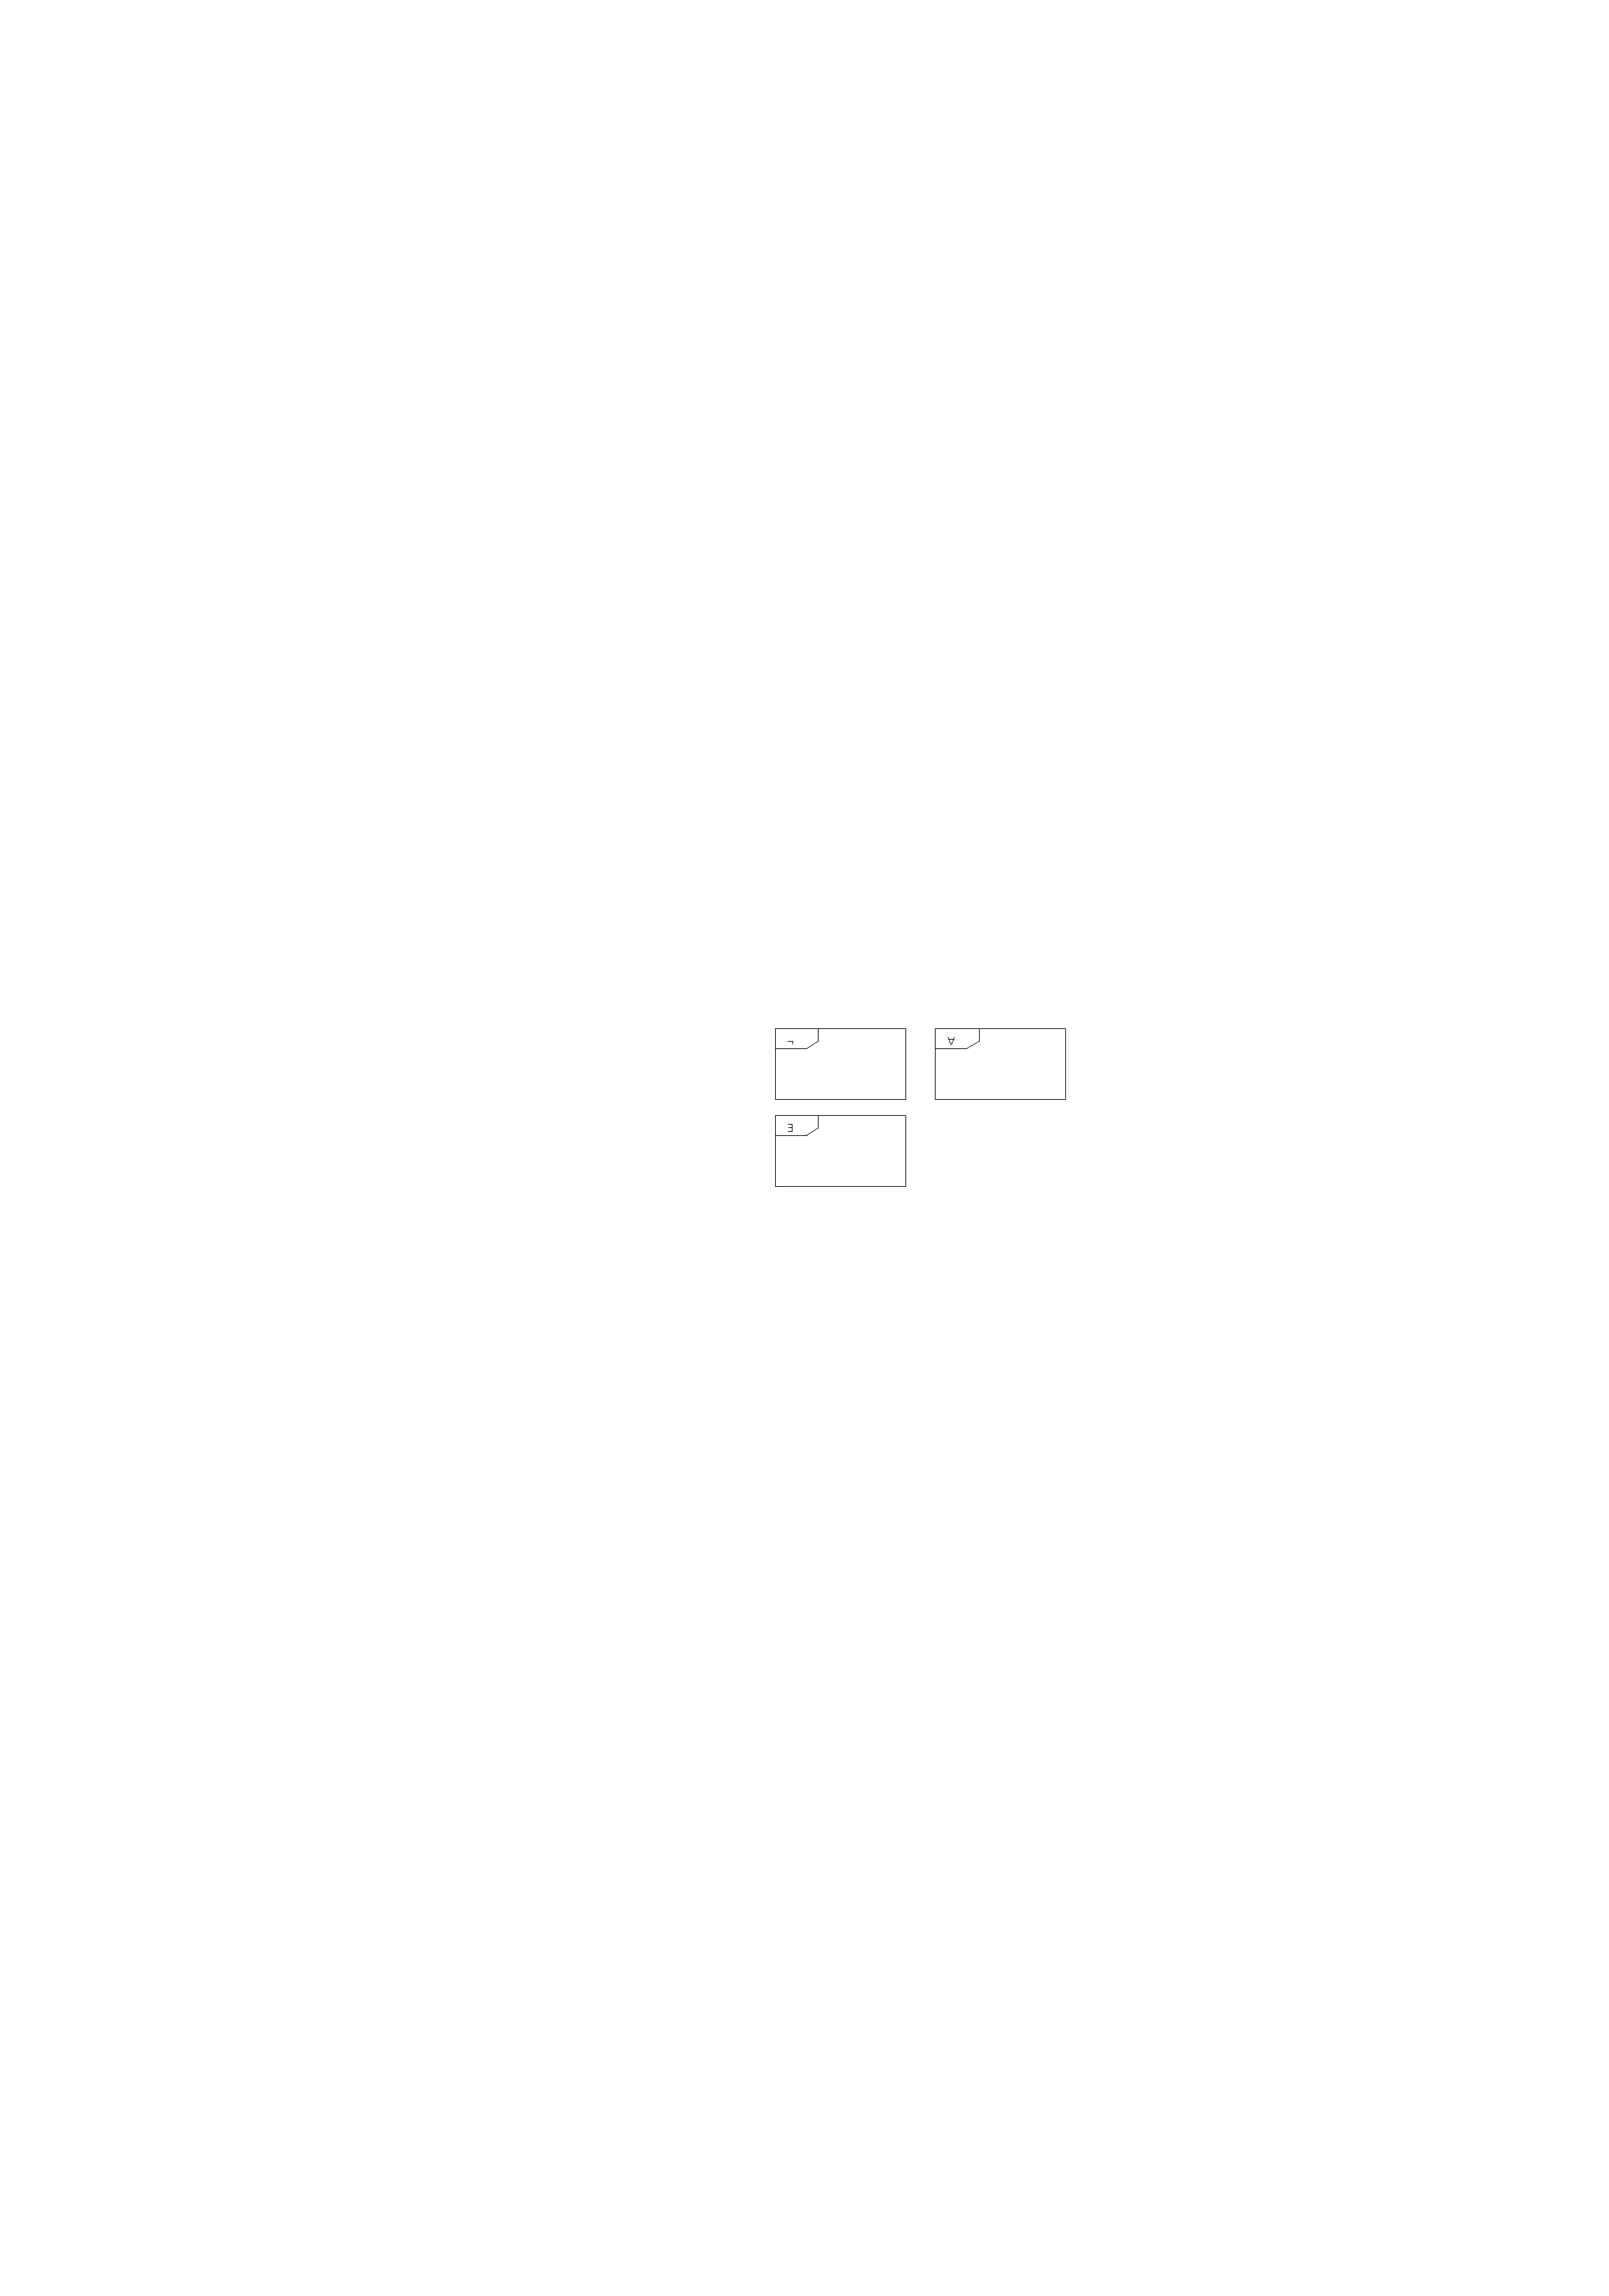
\includegraphics[scale=1.0]{figures/ContainedPattern}
  \caption{Different Kinds of Contained Patterns}
  \label{fig:containedPattern}
\end{figure}

\todomcp{Should contained pattern be marked as optional? Is currently possible in the metamodel. Idea for semantics: Whole pattern must be found, if found, variables may be used in subsequent activities, if pattern may not be found as a whole, matching still succeeds but all variables in the subpattern are not bound in subsequent activities.}
\tododt{I would say, contained patterns are mandatory in general (or are NAC/optional/set in case of the according fragment).}

\begin{figure}[htbp]
  \centering
  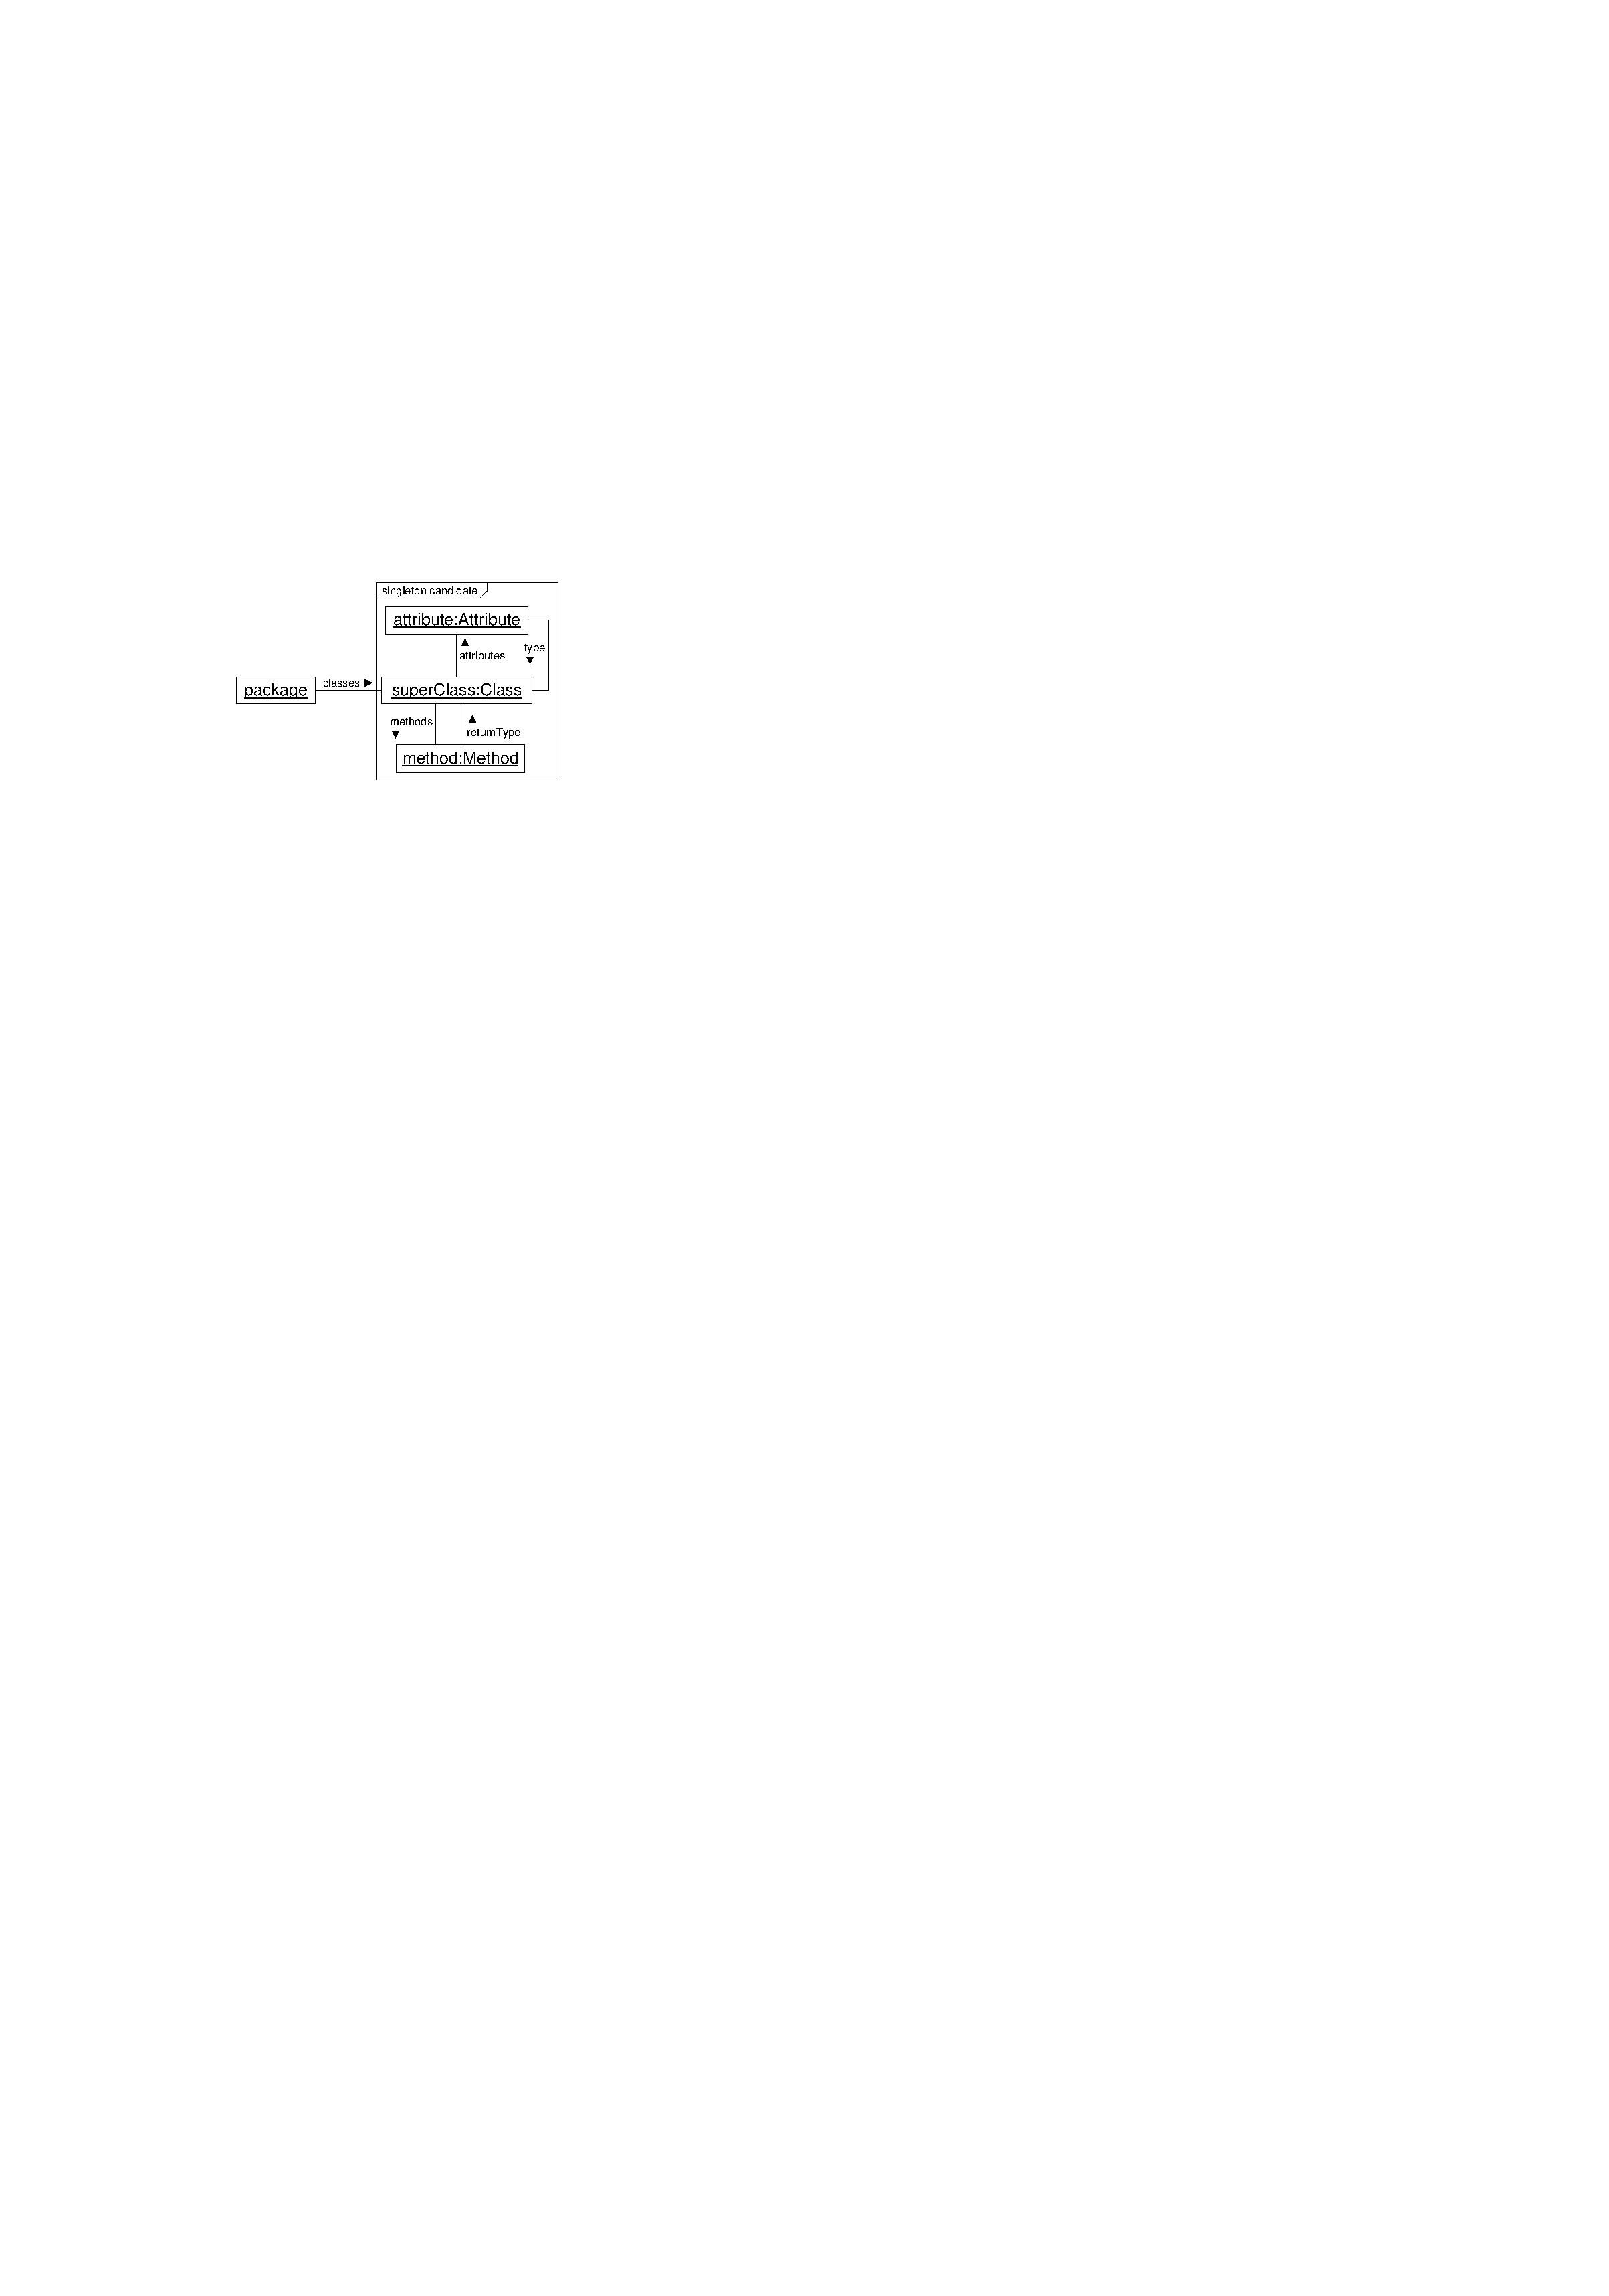
\includegraphics[scale=1.0]{figures/SubPatterns2}
  \caption{Labeled sub pattern}
  \label{fig:labeledSubPattern}
\end{figure}

\begin{figure}[htbp]
  \centering
  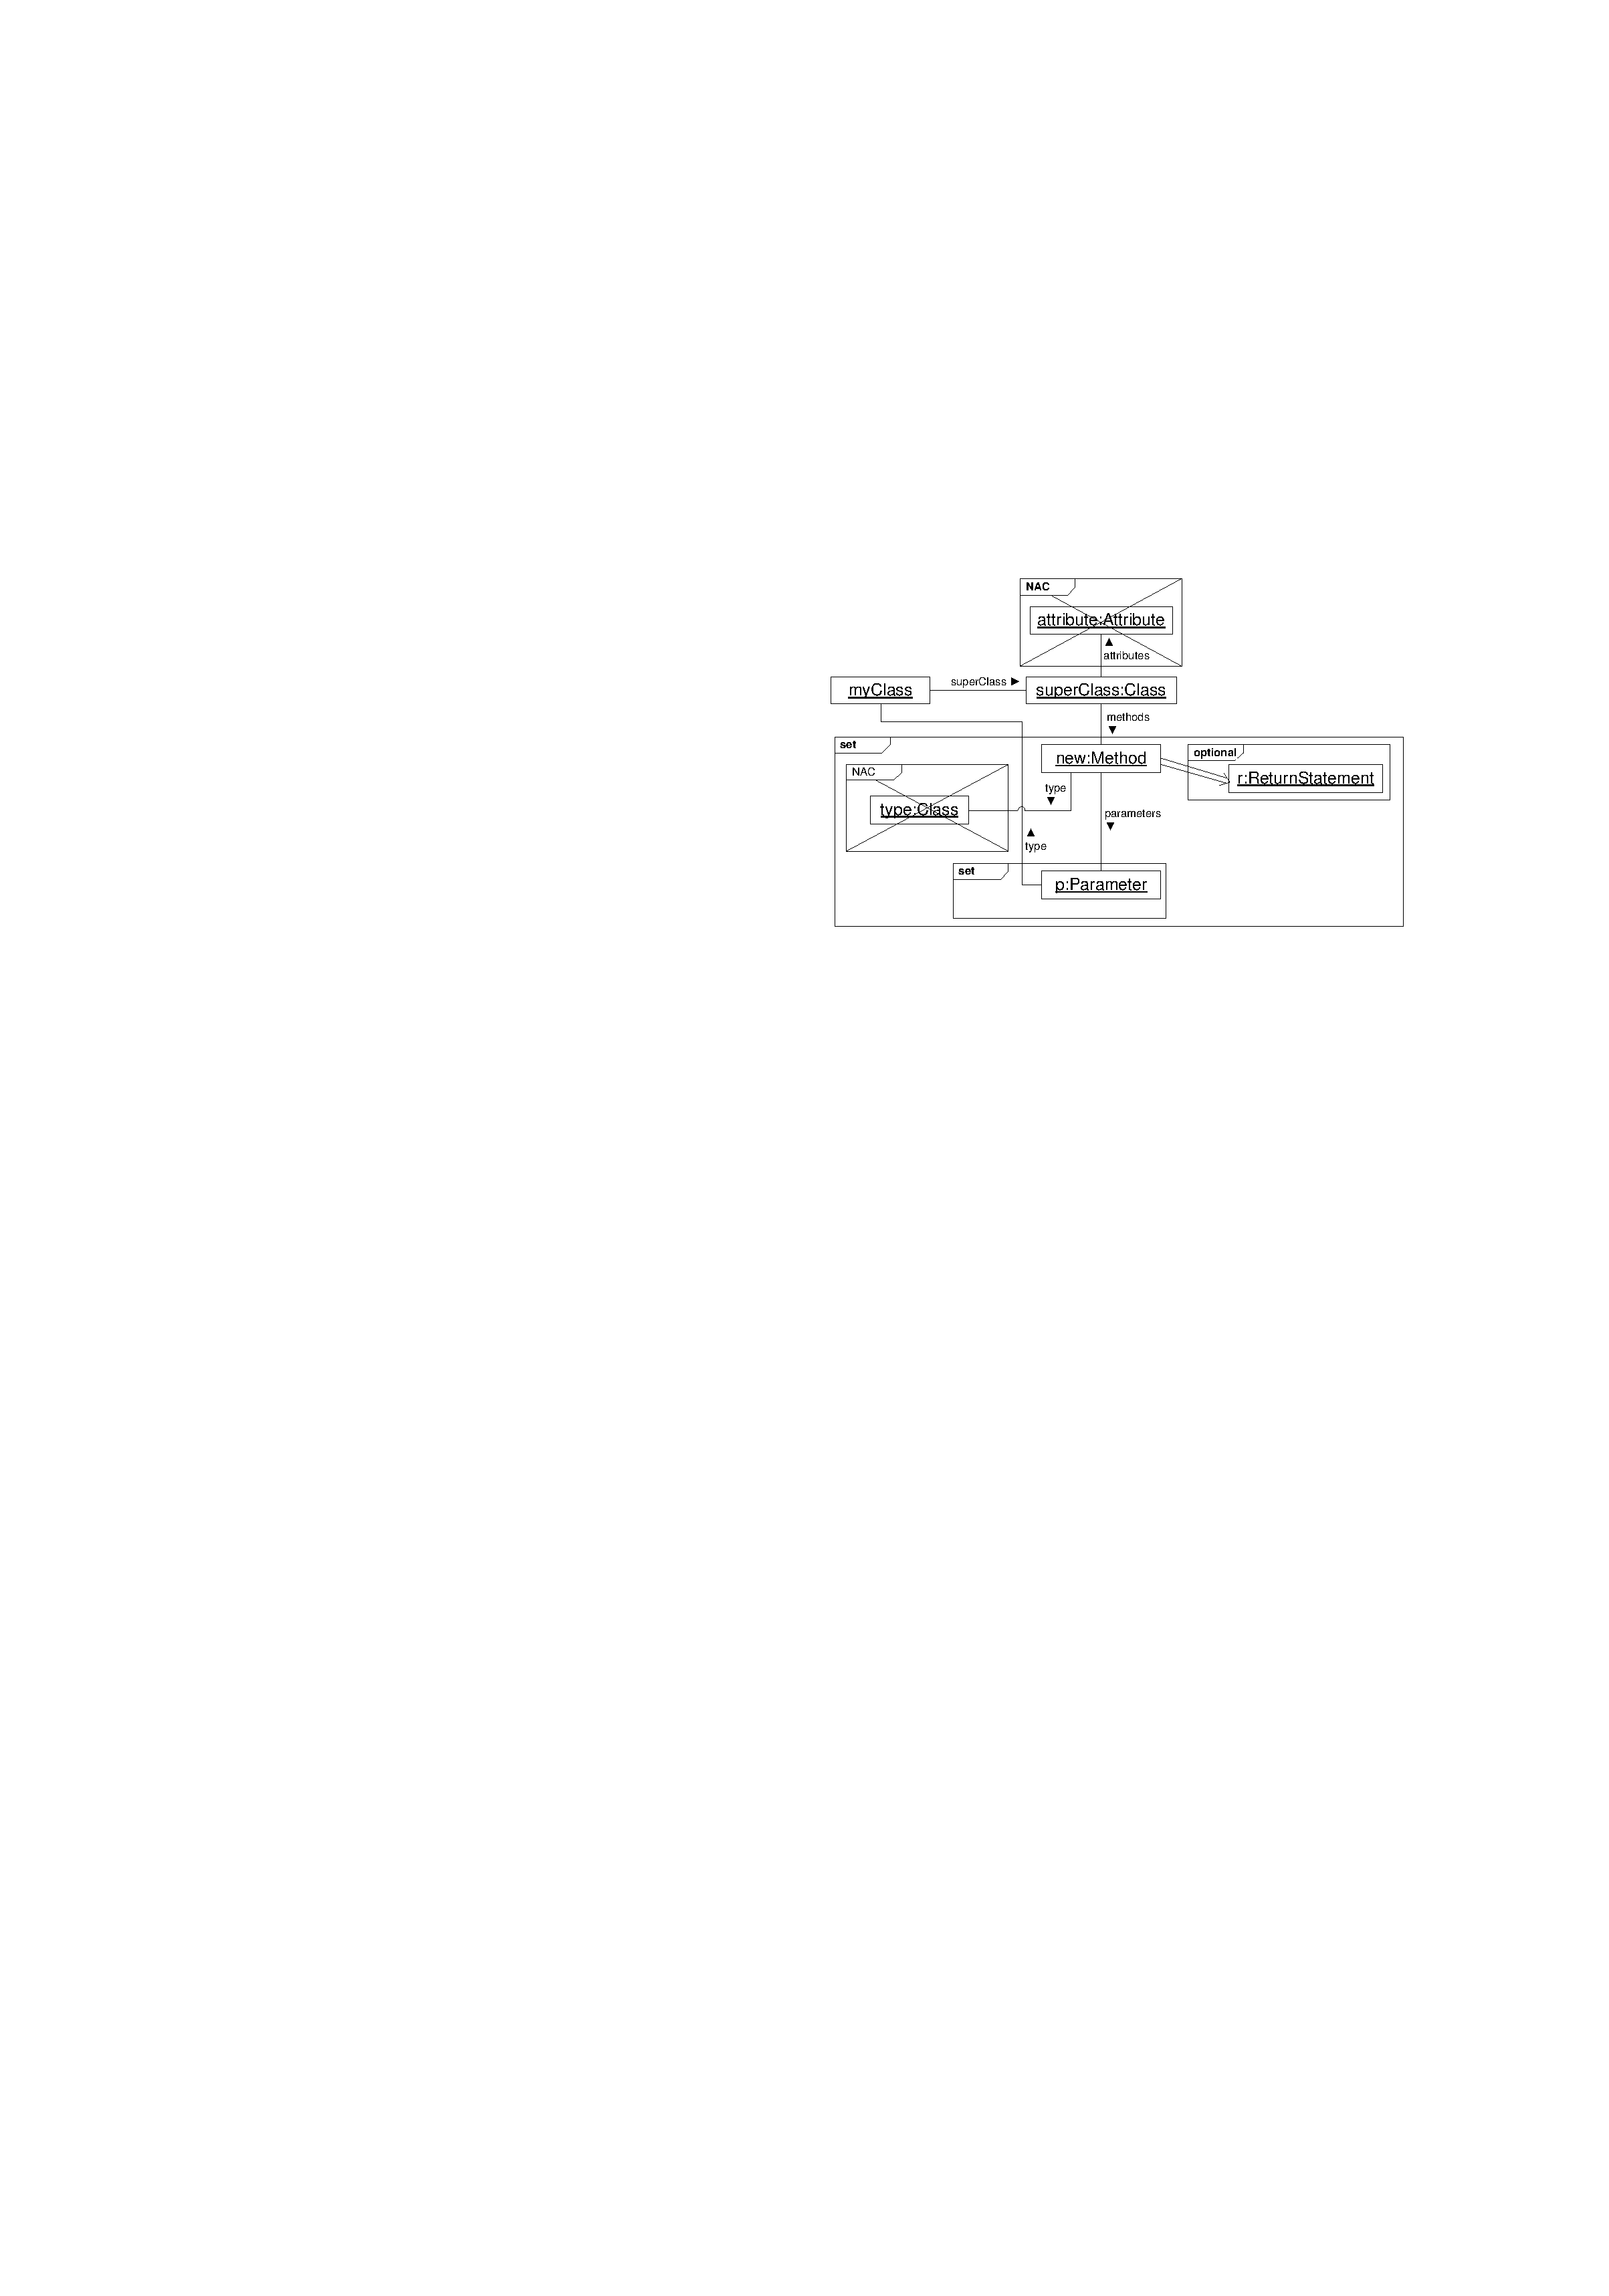
\includegraphics[scale=1.0]{figures/SubPatterns1}
  \caption{Hierarchies of NAC, set, and optional sub patterns}
  \label{fig:subPatternHierarchies}
\end{figure}

\todomcp{How deep may patterns be nested? What is the semantics of alternating binding semantics of sub-patterns, e.g. negative in optional in negative and so on.}
\tododt{I would prefer to allow arbitrarily deep nestings and would suggest to interpret the fragments in the order from outside to inside. Example (see Figure~\ref{fig:subPatternHierarchies}): You match a super class \emph{superClass} of \emph{myClass} and ensure that \emph{superClass} has no attribute. Then you you match all methods \emph{new} (outer set fragment) that have no class as their type (enclosed NAC fragment). Now you match for each of these methods all parameters (enclosed set fragment) that have \emph{myClass} as their type. Furthermore, you try to find a path from the matched \emph{new} method to a return statement (optional fragment).}

} %--- End of pattern fragment section


